\documentclass[letter,12pt]{article}
\usepackage[letterpaper,right=1.25in,left=1.25in,top=1in,bottom=1in]{geometry}
\usepackage{setspace}

\usepackage[utf8]{inputenc}   % allows input of special characters from keyboard (input encoding)
\usepackage[T1]{fontenc}      % what fonts to use when printing characters       (output encoding)
\usepackage{amsmath}          % facilitates writing math formulas and improves the typographical quality of their output
\usepackage{url}              % adds line breaks to long urls
\usepackage[pdftex]{graphicx} % enhanced support for graphics
\usepackage{tikz}             % Easier syntax to draw pgf files (invokes pgf automatically)
\usetikzlibrary{arrows}

\usepackage{mathptmx}           % set font type to Times
\usepackage[scaled=.90]{helvet} % set font type to Times (Helvetica for some special characters)
\usepackage{courier}            % set font type to Times (Courier for other special characters)

\usepackage[longnamesfirst, sort]{natbib}\bibpunct[]{(}{)}{,}{a}{}{;} % handles biblio and references 

\usepackage{rotating}         % sideway tables and figures that take a full page
\usepackage{caption}          % allows multipage figures and tables with same caption (\ContinuedFloat)

\usepackage{dcolumn}          % needed for apsrtable and stargazer tables from R to compile
\usepackage{arydshln}         % dashed lines in tables (hdashline, cdashline{3-4}, 
                              %see http://tex.stackexchange.com/questions/20140/can-a-table-include-a-horizontal-dashed-line)
                              % must be loaded AFTER dcolumn, 
                              %see http://tex.stackexchange.com/questions/12672/which-tabular-packages-do-which-tasks-and-which-packages-conflict


\newcommand{\mc}{\multicolumn}

\begin{document}

\title{Congress skips its turn, again: \\ Agenda obstruction in Chile's Congress\thanks{The author is grateful to José Antonio Cheibub, Gisela Sin, and participants at the Comparative Politics Workshop of the University of Illinois at Urbana-Champaign for useful comments and critiques; to the Department of Political Science at Washington University in St.\ Louis, where much of this work was done as visiting scholar; and acknowledges financial support from the Asociaci\'on Mexicana de Cultura A.C.\ and CONACYT's Sistema Nacional de Investigadores. The author bears sole responsibility for mistakes and shortcomings in the paper.}}
\author{Eric Magar \\ ITAM }
\date{\today}
\maketitle

\begin{center} \textbf{$\rightarrow$~~Preliminary draft~~$\leftarrow$} \\ (please inquire for new version, \small{\url{emagar@itam.mx}})  \end{center}

\begin{abstract}
\noindent Unlike presidents with mostly (or only) reactive formal powers in the legislative arena, Chile's enjoys formidable proactive ones. One is the urgency authority. A bill declared urgent confronts the chamber with a short deadline to discuss and vote it. Urgency, research has shown, improves the odds of bill passage, and most executive-initiated legislation becomes urgent at some stage. I investigate the decision to declare or not legislation urgent, an aspect that has received less scholarly attention. Analysis of original data distinguishes messages in the 1998--2014 period that set forth urgency (40\% of 20 thousand), messages that changed the deadline (29\%), and messages to withdraw the bill's urgency (31\%). Isolating bill and session traits that correlate with urgencies sheds light on the president's power to constantly obstruct the legislative agenda and its use in executive-legislative negotiation with separation of power.  
\end{abstract}

\onehalfspacing

The book has sought to show that the generic, often tacit, and quite ubiquitous model of politics in presidential systems is too simple. That model portrays a president and Congress with shared policy-making power as engaged in an ultimatum game. That one side proposes something that the other accepts or rejects is, indeed, a fundamental trait of the system. But, leaving other important elements aside, the model has lead to a dichomotomous view of gridlock/not that has been inimical to an understanding of decision-making in separation of power systems in comparative politics.

Previous chapters highlight elements that interact in decision-making with the branches' mutual veto. Adding ``minor'' institutional detail (Can vetoes be overridden? Can anyone move unilaterally?), motivation (Are politicians policy-oriented only? Does it matter?), or strategic considerations (Why move if you anticipate a rejection?) greatly sharpens the model's explanatory power. 

%In a world of expanded government responsibilities, ``the need for coordinated and coherent programs, legislative as well as administrative, has become paramount'' \citep[][:4]{apsa.1950}. 

This chapter continues the exploration of unilateralism in presidential systems with an inspection of the urgency authority. Five Latin American constitutions give the executive power to interfere, to some degree, with the assembly's voting schedule. The urgency authority varies considerably \citep[][:437]{morgenstern.2002b}. In Brazil, the assembly must act on a bill deemed urgent withing 45 days, or else it takes precedence over all other legislative business. All executive unilateral policy (\emph{medidas provis\'orias}) become urgent upon publication since 2001. In Colombia, an urgent bill goes to the top of the voting schedule immediately. In Uruguay and Chile, legislators must act withing a pre-specified, short period; failure to do so converts the urgent bill into law in Uruguay. In Chile the consequences of inaction are indetermined. And in Mexico since 2012, the president can declare urgent up to four bills every year, which must be scheduled for a floor vote within 30 days. 

Interfering with the legislative schedule does not end policy differences between the branches per se, and the urgency authority confronts a paradox. Can it convey influence in the legislative arena? Given an urgency, a recalcitrant assembly will simply stop the president's proposal sooner then it would have done. But at least two differences become plainly evident: the timing, whatever had been prioritized by assembly leadership is inevitably pulled down in the schedule by executive fiat; and the action, as legislators will be forced to explicitly bring down the proposal, instead of letting it stand (perhaps indefinitley). Such difference, this chapter aims to show, may put pressure on the legislature and therefore serve as an alternative form of negotiation. This opens up new facets in executive-legislative negotiation. 

The paper offers a preliminary inspection of the urgency authority and its use in Chile since 1998. Section 1 reviews the formal institution and twin studies that have inspected some of its consequences. Section 2 offers sketches that could help produce a theory of the urgency authority. Two elements are highlighted, how the urgency changes the salience of policy and the visibility of rejecting it, and how legislators' impatience might be exploited by the executive. Section 3 describes an original dataset of bill histories and urgency messages in Chile in the 1998--2014 period. The description of  bill initiation, bill passage, and urgency use produce patterns that open a set of questions that could/should be addressed by a systematic study of unilateralism in Chile. Section 4 pays attention to committee reporting, one step of the process that should be influenced by urgency messages that can be measured with the data. The section confirms that, despite institutional ambiguity, the urgency authority makes an imprint in the legislative process. Section 6 carries a very preliminary study of some determinants of urgency authority use in the period. There is no conclusion, but comments and critiques are very welcome to help me push this investigation to the next level. 


\section{The urgency authority}

Formal executive authority to interfere in the Congressional agenda is established in the Constitution (art.\ 74) and Congressional Organic Law (arts.\ 26 and 27). The constitution stipulates that the president can urge action on any bill at any stage of the legislative process. The chamber receiving the urgency message is compelled to act on the bill (``discuss and vote it'') before a specific deadline. Since inter-cameral differences are dealt with in conference (\emph{comisión mixta}, const.\ arts.\ 68--70), an urgency message at this stage compells Congress (ie.\ the conference and both chambers) to act before the deadline. The law defines the breadth of the interference, giving the president a choice of sending a `four-week notice' (\emph{urgencia simple}), a `two-week notice' (\emph{urgencia suma}), or an `act now' (\emph{discusión inmediata}) message.\footnote{In July 2010, when the constitution was amended, the deadlines for the act-now and two-week urgencies were somewhat relaxed, stretching from 10 to 15 and from 3 to 6 days, respectively; four-week urgencies stayed put, at 30 days.} Raising maximum urgency in the right circumstances---an act-now message attached to a bill in bicamernal conference before 2010---gave each instance a single day to act: one for the conference to report a compromise bill, and one for each chamber to sequentially evaluate and push the bill to the floor for an up or down vote (congressional practice is well summarized by the library of Congress at \url{http://www.bcn.cl/ecivica/formacion/}.) The president can retire the urgency at will, with immediate effects. Urgencies affect business in the chamber receiving the message only (*confirm this), and they expire at the end of the ordinary period on March 10th every year. 

Vagueness surrounds key aspects of the urgency authority. When a 3- or 6-day limit is established, are those business or calendar days? I refer to the messages in weeks given indefinition about this (and, when coding deadlines in the empirical sections below, arbitrarily rely on business days). More important, what if Congress fails to act on an urgent bill before the deadline? More specifically, what is the reversion agenda and/or policy if Congress ignores an urgency message?\footnote{How is the day's order (\emph{tabla}) prepared in each chamber? Investigating scheduling in each chamber should illuminate the question. The Constitution and Organic Law remain silent about it.} 

The importance of the issues left obscure is such that the possibility that the urgency authority has no effect cannot be ruled out. The empirical assessment below suggests that this is far from being true in Chile. 

%What if Congress fails to act? Can urgency be ignored? Can a committee report kill the bill or does urgency compell a vote in the floor (law's art.\ 27 ``su discusión y votación en la Cámara requerida deberán quedar terminadas en el plazo'')?

The urgency authority has received relatively scant scholarly attention. In a piece putting Chilean executive-legislative relations in perspective, \citet{siavelis.2002} hypothesized urgencies' game-changer potential. Data covers the first post-transition presidency only, yet revealed just how very frequently urgency messages are sent to Congress, *numbers. Analysis sought to discover if urgent bills circulated the steps of the legislative process faster. Such pattern is clearly distinguishable for act-now urgencies, but not for the other kind, durations here. 

Another systematic study of the urgency authority is \citet{aleman.navia.UrgChi.2009}. The piece concentrates on presidential proposals only up to 2006, seeking determinants of passage. The units are individual bills, and the size of the executive agenda varies substantially over the years. Variation is quantitative (numbers up, down here) and qualitative, presidents manifesting different propensities to aim at constitutional reform. Of direct relevance are the findings on urgencies. Controlling for key policy domains, chamber of origin, seat margins, and presidential approval, and clustering errors by legislative year, different prioritization reveal quite different effects in passage. Act-now and 2-week notices significantly increase the probability of bill passage, but not 4-week notices. 

Selection problems complicate analysis considerably, something that my exploratory analysis, like the Siavelis and Alemán-Navia studies, recognizes but does not confront. The relevant quantity of interest is whether the use of the urgency authority affects bill passage (success, speed, amendments, and so forth) compared to the same bill with no urgency attached. The fundamental problem of causal inference is immediately evident. The executive presumably targets bills for urgency strategically, so that the selection mechanism cannot be assumed random. If, for example, more complex and divisive legislation takes longer, is likelier to fail and likelier to be tagged urgent, separating effects requires more subtle methods than used up to now.

Exploratory analysis in this work does not address the selection problem. It will search for determinants of urgency authority use, in the hope of paving the way for a solution. The research design should change to attempt a solution. 

\section{Elements for a model of the urgency}

Urgency authority lets executives force action on legislation, more or less immediately. But a legislature acting on a proposal is not equivalent to adoptioninto law. Declaring a bill opposed by the majority urgent may only hasten its rejection. So isn't the urgency authority doomed to begin with? Can an executive with such authority negotiate better with an opposition assembly than one without urgency auhtority? Under what circumstances? This section sketches elements to address this puzzle. 

% \citet{carey.shugart.1998a} offer clues on the delegation of unilateral authority to the executive. Latin American presidents have much more valence on policy than legislators \citep{londregan.2000a}, and such informational asymmetries may create incentives for delegation. Delays to reach agreement may also diminish the value of policy \citep{baron.ferejohn.1989}, so rather than delegate proposal power within the chamber, legislators may prefer to see the president set the agenda. Agency costs will be determinant on the actual prevalence of such forms. When set constitutionally, as Chile does, there is no alternative. 

% This section highlights other elements that should be of help in building a model of urgencies. I elaborate on two possible uses of the urgency: when rejection is costly and when there is impatience. Forcing rejection of a proposal might activate costs in units other than policy. Changing the nature of what is being negotiate might, in fact, trigger policy concessions. (Similar a vetoes with Q=.5). Another use s to exploit impatience when time is a constrain. Avoiding agenda obstruction may, again, offer the executive a bargaining chip. 

\subsection{Costly scheduling and inaction}

Five constitutions of the Americas give executives the power to interfere, to some degree, with the assembly's voting schedule. The urgency authority varies considerably \citep[][:437]{morgenstern.2002b}. In Brazil, the assembly must act on a bill deemed urgent withing 45 days, or else it takes precedence over all other legislative business. And, since 2001, all executive unilateral policy (\emph{medidas provis\'orias}) become urgent upon publication. In Colombia, an urgent bill goes to the top of the voting schedule immediately. In Uruguay and Chile, legislators must act withing a pre-specified, short period; failure to do so converts the urgent bill into law in Uruguay. In Chile the consequences of inaction are indetermined. And in Mexico since 2012, the president can declare urgent up to four bills every year, which must be scheduled for a floor vote within 30 days. 

\begin{figure}
  \centering
    \tikzstyle{mid}=[circle,draw]
    \begin{tikzpicture}
      \node[mid] at (2,0) (e) {\emph{E}}; 
      \node[mid] at (4,1) (l) {\emph{L}}; 
      \node[right] at (4,-1) (ee) {$x_0$}; 
      \node[right] at (6, 2.5) (le1) {$x_1-o$};  
      \node[right] at (6, 1) (le3) {$x_0-o-c_1$}; 
      \node[right] at (6,-.5) (le2) {$r-c_2$}; 
      \path[-]  (e) edge node [above, sloped] {\footnotesize{propose}} (l);
      \path[]   (e) edge node [below, sloped] {\footnotesize{$x_1$}}   (l); 
      \path[-o] (e) edge node [below, sloped] {\footnotesize{not}}     (ee) 
                 (l) edge node [above, sloped] {\footnotesize{accept}} (le1) 
                 (l) edge node [below, sloped] {\footnotesize{ignore}} (le2);
      \path[-o] (l) edge node [above, sloped] {\footnotesize{reject}} (le3);
    \end{tikzpicture}  \begin{tabular}{lrrr}
  Case                       & $r$   & $c_1$ & $c_2$    \\ \hline
  Chile                      & $x_0$ & 0     & $>0$     \\
  Brazil (urgency), Colombia & $x_0$ & 0     & $> o$ \\
  Brazil (MP)                & $x_0$ & $>0$  & $> o$ \\
  Brazil (MP up to 2001)     & $x_1$ & $>0$  & 0        \\
  Mexico                     & $x_0$ & 0     & ?        \\
  Uruguay                    & $x_1$ & 0     & 0        \\
  \end{tabular}
  \caption{Urgency and costly scheduling and rejections. }\label{f:costly}
\end{figure}

Figure \ref{f:costly} offers a framework to compare different urgency authorities. It is set as a two-player game between the executive and the pivotal legislator. The executive starts by proposing urgent policy $x_1$, or not (ending the game with the status quo $x_0$ in place). Initially, costs $c_1 = c_2 = 0$ so that they cancel from the description, for ease of exposition. The restriction is relaxed afterwards. If called to play, the legislator faces three actions to choose from, all leading to terminal nodes. The legislator can accept the proposal, replacing the status quo with policy at $x_1$. Given scarce scheduling time, this choice entails an opportunity cost $o$. Conceptually, cost $o$ is the value of the best alternative policy that the legislator might adopt if scheduled instead of proposal $x_1$. With scarce time, and an institution that no two (or more) proposals are scheduled simultaneously, putting $x_1$ to a vote inevitably postpones the adoption of the alternative---indefinitely, perhaps. Cost $o$ must therefore be deducted from the value of policy $x_1$ in the top terminal node (the figure expresses costs from the legislator's perspective). The legislator could alternatively choose to keep the status quo by rejecting the proposal. Cost $o$ must also be deducted in this case due to the need to schedule the bill in order to vote it down in the floor. And the legislator could opt to ignore the proposal, policy reverting to a pre-defined reversion outcome $r$. Unlike the other two alternatives, ignoring the proposal spares cost $o$: time is freed to schedule something else. 

Reversionary policy $r$ varies across constitutions, adopting either the status quo ante or the proposal. The Uruguayan reverts policy to executive proposals declared urgent but not scheduled for a vote (i.e., $r=x_1$); the rest revert to the status quo ante ($r=x_0$)---although the Brazilian compared to the Uruguayan in cases of urgency by \emph{medida provis\'oria} up to the 2001 reform.\footnote{\emph{Medidas provis\'orias} expire 60 days after publication. Before the reform, a Supreme Court ruling legalized the option of re-issuing MPs that had not been discussed and voted in Congress upon expiration, leading to the instituion described in the text ($r=x_1$). The reform adopted 9/11/2001 limits to one re-issue, with urgency kicking in in case of congressional inaction. See \citet{figueiredo.etal.1996}.} When $r=x_0$, all else equal, the legislator prefers to ignoring rather than rejecting undesirable proposals, so as to avoid opportunity costs (this claim ignores the possibility of $o<0$). Jibes with evidence, report. The other institution $r=x_1$ results in a drastic change in executive--legislative relations, as congressional inaction becomes a way of adopting presidential policy without opportunity cost.  

Relaxing the restriction of nil costs other than $o$ brings further depth into the comparative framework. I highlight three elements making such costs distinct from zero: diffuse support becoming concentrated, salience, and from scheduling interference.

The first is associated with unilateralism, which is associated with the urgency authority in Brazil only (executive unilateralism per se, though, is present in other constitutions). \emph{Medidas provis\'orias} turns potential into actual winners and losers. At the proposal stage, there is an expectation that a group might receive a flow of benefits if all goes according to plan. All is surrounded by a fair amout of uncertainty, both about the likelihood that policy will in fact materialize and about the scope of benefits associated with the details of the policy that eventually passes. Once adopted, this uncertainty vanishes. When policy is adopted unilaterally, winners and losers are clearly identified before the measure is discussed and voted, changing the assembly's calculus. Rescinding the decree will face an opposition that is easily identifiable. This translates into a cost.  

The salience component derives from the very notion of urgency. Labeling a proposal thus signals presidential priority. Coupled with a clever communication strategy, the urgency authority contributes to placing an issue in the public agenda, increasing media attention and nurturing public debate. An undesired proposal that could have easily been dusted under the carpet in normal circustances will, as a consequence of increased salience, be much harder to duck---adding a cost. 

Scheduling interference adds a substantal cost when the institution brings an urgent proposal to the top of the assembly's Day's Order. At this point, ignoring proposal $x_1$ not only will not spare opportunity cost $o$, but scheduling the proposal becomes more attractive in order to pay $o$ in one session only, and move on to the next item in the agenda. Scheduling interference also adds costs in the form of possible splits of your legislative coalition---when the urgency authority brings forth to a vote issues that majority leaders would rather keep away from the floor. 

The table accompanying Figure \ref{f:costly}'s game tree summarizes costs other than $o$ associated with rejection and ignoring the proposal in the five constitutions. A non-zero rejection cost $c_1$ adds to the opportunity cost in case of urgencies stemming from executive unilateral action only (fighting concentrated opponents). Ignoring cost $c_2$ remains nil in Uruguay and remained so in Brazil before the 2001 reform (inaction reverts to $r=x_1$ automatically). In Mexico, the consequences of inaction are indeterminate. Perhaps a future Supreme Court ruling or legislation will fill in the blanks. In Chile, a $c_2>0$ will be a direct function of how salient the proposal becomes upon raising the urgency. I discuss below how qualifying the urgency---as the constitution allows---generates expectations on the level of salience. In Colombia and post-reform Brazil, $c_2$ surpasses opportunity cost $o$ in light of scheduling interference (cost $o$ is paid in every session that the legislator opts for inaction). 

--> Next, discuss Chile in detail. Tie salience to degree of urgency, showing that `Act now' is muche less used. 

--> Hypotheses about div gov: cartel (in one chamber at least) does not have the president on its side, losing key negative agenda control. Makes majority's life much harder. 

--> Connect to frequency of urgency usage; to reports observed and not withing deadline; to roll call votes celebrated. 

--> Regressions on reports

--> Regression on votes?

--> Conclude about the effects of indeterminacy in Chile; announce Brazilian study.

\subsection{Visibility}

All majorities are the sum of minorities. Group or party members share goals, often many, but never all. Coalition and party leaders know this and will normally attempt to avoid deciding on issues with potential to split the coalition \citep{riker.1986,shepsle.2003}. A majority's failure to control the agenda thus runs many risks, chief among them being rolled if the splitting faction gives the opposition enough votes to defeat the motion \citep{cox.mccubbins.2005}. A problem therefore arises when negative agenda control (leaving items off at will) is less than perfect. 

Stylizing rejection of undesirable policy as entailing a cost reveals one aspect of imperfect agenda control. Such cost comes in a different currency than policy. A conservative party voting to curb immigration risks alienating conservative immigrants, and voting against risks alienating nativists. If young immigrant conservatives were key to the well-being of the party, immigration curbs would entail electoral costs $c<0$ in the foreseeable future. Prudent leaders might therefore prefer to duck the question, keeping it off the agenda, and thus prevent a vote. The best option remains to fail to schedule the divisive discussion and vote, silently retaining the status quo without paying rejection penalties. 

\begin{figure}
  \centering
  % \begin{tabular}{cc}
  %   (a) No urgency power & (b) Proposal declared urgent \\
    \tikzstyle{mid}=[circle,draw]
    \begin{tikzpicture}
      \node[mid] at (2,0) (e) {\emph{E}}; 
      \node[mid] at (4,1) (l) {\emph{L}}; 
      \node at (4,-1) (ee) {$x_0$}; 
      \node at (6.5,2.5) (le1) {$x_1$};  
      \node at (6.5,1) (le3) {$x_0$}; 
      \node at (6.5,-.5) (le2) {$x_0$}; 
      \node[right] at (4.25,-1) {\footnotesize{$(0)$}};  
      \node[right] at (6.75,2.5) {\footnotesize{$(b)$}};  
      \node[right] at (6.75,1) {\footnotesize{$(0)$}};  
      \node[right] at (6.75,-.5) {\footnotesize{$(c)$}};  
      \path[-] (e) edge node [above, sloped] {\footnotesize{propose}} (l);
      \path[] (e) edge node [below, sloped] {\footnotesize{$x_1$}} (l); 
      \path[-o] (e) edge node [below, sloped] {\footnotesize{not}} (ee) (l) edge node [above, sloped] {\footnotesize{accept}} (le1) (l) edge node [above, sloped] {\footnotesize{pay to}} (le2) (l) edge node [below, sloped] {\footnotesize{reject}} (le2);
      \path[-o, dashed] (l) edge node [above, sloped] {\footnotesize{ignore}} (le3);
    \end{tikzpicture}
  %   & 
  %   \tikzstyle{mid}=[circle,draw]
  %   \begin{tikzpicture}
  %     \node[mid] at (2,0) (e) {\emph{E}}; 
  %     \node[mid] at (4,1) (l) {\emph{L}}; 
  %     \node at (4,-1) (ee) {$x_0$}; 
  %     \node at (6.5,2.5) (le1) {$x_1$};  
  %     %\node at (6.5,1) (le3) {$x_0$}; 
  %     \node at (6.5,-.5) (le2) {$x_0$}; 
  %     \node[right] at (4.25,-1) {\footnotesize{$(0)$}};  
  %     \node[right] at (6.75,2.5) {\footnotesize{$(b)$}};  
  %     %\node[right] at (6.75,1) {\footnotesize{$(0)$}};  
  %     \node[right] at (6.75,-.5) {\footnotesize{$(-c)$}};  
  %     \path[-] (e) edge node [above, sloped] {\footnotesize{propose}} (l);
  %     \path[] (e) edge node [below, sloped] {\footnotesize{$x_1$}} (l); 
  %     \path[-o] (e) edge node [below, sloped] {\footnotesize{not}} (ee) (l) edge node [above, sloped] {\footnotesize{accept}} (le1) (l) edge node [above, sloped] {\footnotesize{pay to}} (le2) (l) edge node [below, sloped] {\footnotesize{reject}} (le2);
  %     %\path[-o] (l) edge node [above, sloped] {\footnotesize{ignore}} (le3);
  %   \end{tikzpicture}
  %  \\
  % \end{tabular}
  \caption{Costly rejections. Parentheses right of outcomes are the legislator's gain vis-\`a-vis the status quo.}
\end{figure}

The urgency authority makes it harder, or even impossible, to exert negative agenda control, and the game in Figure \ref{f:costly} highlights how this matters. The executive starts by proposing new policy $x_1$ or not (ending the game with the status quo $x_0$ in place). New policy necessitates the legislator's approval. The game tree contemplates two ways of reinstating the status quo after a proposal the legislator disagrees with has been made: by rejecting it, or by ducking the question (the dashed branch in the game tree). Explicit rejection entails a cost $c$ for the legislator, which is avoided by ignoring the issue. That large numbers of proposals in assemblies worldwide are never scheduled for consideration is consistent with the presence of non-zero rejection costs. 

Parentheses in the figure report the legislator's payoffs as gains against the status quo. Outcome $x_0$ in two of three terminal nodes accordingly has payoff zero because there is no change. The exception is explicit rejection, when the rejection cost must be netted from the nil payoff. And $b$ stands for the legislator's gain (which may be negative, just like costs can be positive) of accepting the executive proposal. 

`Ignoring' strongly dominates `rejecting' the proposal whenever $c<0$. But a binding urgency message, however, changes the game structure by removing the dashed branch from the game tree---the urgent proposal can no longer be ignored, it must be voted down at cost $c$. 

This preliminary discussion of a simple game shows how, in the absence of costs associated with rejecting proposals, no room remains for policy $x_1$ to survive against the legislator's opposition ($b<0$). But big-enough costs ($c<b$) push the legislator to accept proposals she would otherwise reject. Costly rejection translates into accommodation, a policy advantage that no strategic executive will fail to exploit. 

%The presence of a cost c makes the use of decrees more interesting, while keeping the amplified sop game simple.  The simplicity of the sub-game's structure is not so much relative to the other sub-games of the parent super-game---though this surely is the case---than relative to other conceivable structures of formal executive decree authority.  I will devote part of chapter 4 to sketch an alternative model of executive decree authority, more in line with the processes of decree-writing, amending, and erasing actually mandated by the Argentine and other constitutions.  A more elaborate model should also include some parameter to make policy by decree less desirable for the executive than the exact same policy issued by statute---perhaps, as I will argue in chapter 5, because decrees are less robust than statutes.  

%What is the nature of cost $c$?  What determines the size? Are there circumstances when $c>0$?  The cost simplifies what may be a more elaborate structure of policy with unilateral authority.  


\subsection{Impatience}

%FIND FENNO QUOTE TO OPEN THIS SUBSECTION: Short sessions increase the opportunity cost of devoting time to certain issues \citep{fenno.1973}. Rejecting a presidential proposal, and especially if alternative legislation must be drafted, requires investing scarce time from the part of legislators.  

\begin{figure}
  \centering
  % \begin{tabular}{cc}
  %   (a) No urgency power & (b) Proposal declared urgent \\
    \tikzstyle{mid}=[circle,draw]
    \begin{tikzpicture}
      \node[mid] at (-4,0) (el) {\emph{E,L}}; 
      \node[mid] at (-2,0) (l) {\emph{L}}; 
      \node[mid] at (0,0) (e) {\emph{E}}; 
      % \node at (4,-1) (ee) {$x_0$}; 
      % \node at (6.5,2.5) (le1) {$x_1$};  
      % \node at (6.5,1) (le3) {$x_0$}; 
      % \node at (6.5,-.5) (le2) {$x_0$}; 
      % \node[right] at (4.25,-1) {\footnotesize{$(0)$}};  
      % \node[right] at (6.75,2.5) {\footnotesize{$(b)$}};  
      % \node[right] at (6.75,1) {\footnotesize{$(0)$}};  
      % \node[right] at (6.75,-.5) {\footnotesize{$(c)$}};  
      \path[-] (el) edge node [above, sloped] {\footnotesize{propose}} (l);
      \path[]  (el) edge node [below, sloped] {\footnotesize{$(a,b)$,$(e,l)$}} (l);
      % \path[] (e) edge node [below, sloped] {\footnotesize{$x_1$}} (l); 
      % \path[-o] (e) edge node [below, sloped] {\footnotesize{not}} (ee) (l) edge node [above, sloped] {\footnotesize{accept}} (le1) (l) edge node [above, sloped] {\footnotesize{pay to}} (le2) (l) edge node [below, sloped] {\footnotesize{reject}} (le2);
      % \path[-o, dashed] (l) edge node [above, sloped] {\footnotesize{ignore}} (le3);
    \end{tikzpicture}
  \caption{Possib game}\label{f:skip}
\end{figure}


The term urgency points to impatience---wishing results sooner rather than later. I introduce elements showing how impatience on the part of legislators (not the executive, as intuition may suggest) can affect executive-legislative negotiation. The multiplicity of needs from legislators and finite sessions increase the opportunity cost of devoting time to certain issues \citep{fenno.1973}. With enough time constraints, the urgency authority gives the executive another instance to extract concessions from a recalcitrant legislature. 

The approach is decision-theoretic. Extending it to assume strategic behavior should be doable. The legislator and executive have two pet projects each, $a,b$ and $e,f$, respectively. There are two stages to negotiate policy, and only one project can be voted up or down in each period---the rest will have to wait, indefinitely. So, of four separable status quos that may be challenged ($a_0$, $b_0$, $e_0$, and $f_0$), two will prevail---and more if bargaining fails in any stage. To economize, notation for policy also denotes the legislator's associated payoffs. Payoffs are gains vis-\`a-vis the status quo, so that $a_0=b_0=e_0=f_0=0$. As pet projects, it is reasonable to state that $a,b>0$. 

With a time constrain, actors need to prioritize and the agenda becomes critical. Agenda \emph{abef} indicates that $a$ is moved for a vote first, then $b$, then $e$, then $f$---but, with two periods only, negotiation ends before the agenda is exausted. Enter the urgency authority, giving the executive positive agenda power---she can change the agenda unilaterally. Declaring an urgency in round 1 would change the above agenda to \emph{eabf}, and to \emph{efab} declaring another urgency in round 2 as well. 

\begin{table}
\centering
\begin{tabular}{clcc}
Case & Agenda (outcomes)           & Policy             &  Discounted payoff \\ \hline
1    & \emph{abef}~~~(both pass)     & $(a,b,e_0,f_0)$    &  $a + \delta b$    \\
2    & \emph{eabf}~~~($e$ rejected)  & $(a,b_0,e_0,f_0)$  &  $\delta a$        \\
3    & \emph{efab}~~~(both rejected) & $(a_0,b_0,e_0,f_0)$ &  0                 \\
4    & \emph{eabf}~~~(both pass)     & $(a,b_0,e,f_0)$    &  $e + \delta a$    \\  \hline
\end{tabular}
\caption{Agendas, outcomes, and inter-temporal payoffs}\label{T:agendaPayoffs}
\end{table}

A discount factor $0\leq \delta \leq1$ captures impatience, shrinking the value of round 2 policy, and a discounted payoff can be associated to each agenda. Adopting agenda \emph{abef}, the legislator's pet projects are scheduled, which he promptly adopts. Policy in round 1 is $a$ ($b_0,e_0,f_0$, all of value zero, can be ignored, but they are policy as well). In round 2, it is $b$, so applying the discount yields $a + \delta b$ as the agenda payoff (case 1 in Table \ref{T:agendaPayoffs}). 

Absent monopoly agenda control, \emph{abef} may not be a feasible agenda. The urgency authority lets the executive pull forward her own projects, unilaterally setting agenda \emph{efab} for a decision. In case the legislator values policy the president put in the agenda ($e>0$, $f>0$, or both), he should pass one or both proposals. Yet that this comes at the expense of his pet projects is more easily seen with $e,f<0$: the legislator should reject tham both, and status quo policy remains in all four domains---the very puzzle of useless urgency authority. 

But the opportunities foregone bring to bear open a bargaining, gains-from-trade possibility that a strategic extension of the framework might dilucidate. It runs thus: the executive declares her two projects urgent. Then, conditional on passage of $e$ in round 1, the urgency on project $f$ is lifted towards round 2, leaving agenda \emph{eabf} in place of \emph{efab}. In deciding whether or not to accept a deal of this nature, the legislator faces a standard decision calculus. He should accept if the payoff of case 4 in the Table is greater than that of case 3. Formally, because $a>0$

\begin{equation*}
e + \delta a >  0 \iff \delta  >   -\frac{e}{a}.
\end{equation*}

\noindent Since $\delta>0$, with $e<0$ the decision may flip one way or the other depending on the size of the discount factor relative to the values of the pet projects (whenever $e\geq0$ the inequality invariably holds). In general, more impatience (a smaller $\delta$) raises the legislator's willingness to accept executive proposals that he would otherwise reject.  

The decision-theoretic setting fails to address many interesting strategic wrinkles. For instance, when the inequality above fails to point towards accepting a gains-from-trade route, the executive may be better off making concessions ex-ante, moderating her proposal (lowering a negative $e$ in absolute value). It would compensate for the legislator's insuffieicent impatience. But it does point in interesting directions for empirical analysis that a game of this nature could illuminate. 

The discussion so far points to urgency withdrawals, a common phenomenon. According to this perspective, they are not mistakes, or changes in piorities, but bargaining chips. I hold your project hostage until passage of mine. Unlike a priori commitments where promises can be reneged---agendas \emph{aebf} and \emph{eabf} leave open the rejection of $e$ with passage of $a$. The hostage approach makes the legislator's commitment credible---she incurs in a cost for reneging. \citep[Although it is the president's word that is now questionable, she could call $f$ urgent after passage of $e$ to keep $a_0$ in place, cf.][]{weingast.1992}. Commitment credibility should be problematic when the president's party is not in control of the chamber. 

% \begin{table}
% \centering
% \begin{tabular}{cccc}
%       &                   & $A$'s discounted   &  Agenda      \\
% Round & Policy            & gain in round      &  payoff      \\ \hline
% 0     & $a_0,b_0,e_0,f_0$ & 0                  &                                \\ \hdashline
%   \mc{3}{l}{Case 1: agenda \emph{abef} (both pass)}     &  $(1+\delta)a_1 + \delta b_1$  \\
% 1     & $a_1,b_0,e_0,f_0$ & $a_1$              &                                \\
% 2     & $a_1,b_1,e_0,f_0$ & $\delta(a_1+b_1)$  &                                \\ \hdashline
%   \mc{3}{l}{Case 2: agenda \emph{eabf} ($e$ rejected)}  &  $\delta a_1$                  \\
% 1     & $a_0,b_0,e_0,f_0$ & 0                  &                                \\
% 2     & $a_1,b_0,e_0,f_0$ & $\delta a_1$       &                                \\ \hdashline
%   \mc{3}{l}{Case 3: agenda \emph{efab} (both rejected)} &  0                             \\
% 1     & $a_0,b_0,e_0,f_0$ & 0                  &                                \\
% 2     & $a_0,b_0,e_0,f_0$ & 0                  &                                \\ \hdashline
%   \mc{3}{l}{Case 4: agenda \emph{eabf} (both pass)}     &  $(1+ \delta)e_1 + \delta a_1$ \\
% 1     & $a_0,b_0,e_1,f_0$ & $e_1$              &                                \\
% 2     & $a_1,b_0,e_1,f_0$ & $\delta(a_1+e_1)$  &                                \\ \hline
% \end{tabular}
% \caption{Agendas and inter-temporal payoffs}\label{T:agendaPayoffs}
% \end{table}









\section{The data}

Compared to other legislatures in the region, the C\'amara de Diputados' web page (\url{www.camara.cl}), run by the Congressional Library, is remarkably informative and up-to-date. Input a bill's filing number (\emph{boletín}), and any user sees a detailed report with the bill's general traits: who initiated it, when, in what chamber, what it deals with, its status, etc. The report also lists and dates the proposal's milestones in transit through the meanders of the legislative process: committee referral, committee reports to the plenary, floor discussion and voting, navette to the other chamber, etc. It covers milestones in the Senate, too. Of direct relevance, all urgency messages that a bill may have received are listed chronologically. 

An inquiry was sent to the congressional staff in Oct.\ 2014 about the existence of an official API ot FTP site where this well-structured data could be downloaded en bloc. There was no response, so an automated script was prepared (using \texttt{Python}'s Selenium library---the site is javascript-rich) to scrape the web-page. Data analysis was done with a multiplicity of \texttt{R}'s libraries. Details of this script will be posted online. 


\begin{table}
\begin{center}
\begin{tabular}{lrrrrrr}
Coalition   & 1990--94 & 1994--98 & 1998--2002    & 2002--06 & 2006--10 & 2010--14 \\ \hline
\mc{7}{l}{\emph{~~C\'amara de Diputados}} \\
President's & 60       & 58       & 58            & 53       & 51       & 50       \\
Opposition  & 40       & 42       & 42            & 48       & 47       & 48       \\
Regional    &          &          &               &          & 3        & 2        \\ \hdashline
Total       & 100      & 100      & 100           & 100      & 100      & 100      \\ \hline
\mc{7}{l}{\emph{~~Senate}} \\
President's & 48       & 46       & 50            & 50       & 55       & 45       \\
Opposition  & 52       & 54       & 50            & 50       & 45       & 55       \\ \hdashline
Total       & $100^*$  & $100^*$  & $100^{*\dagger}$ & 100      & 100      & 100      \\ \hline
\mc{7}{l}{\footnotesize{Notes: $^*$ vacant seats dropped; $^\dagger$ margin varied above and below 50/50 due to vacancies.}}

\end{tabular}
\caption{The president's status in Congress. Percent seats controlled by electoral lists in each chamber. Between 1990 and 2010, the president's and opposition lists were Concertación and Alianza, respectively; they switched after 2010. The regional list includes splinters from each major list (Christian Democrats and UDI members). Source: prepared by the author with information from the C\'amara's web page at \protect\url{www.camara.cl} (some data kindly shared by Guillermo Rosas).}\label{t:congressSeats}
\end{center}
\end{table}


Analysis covers the 1998--2014 period. Earlier years antedate the internet, and data completeness remains to be verified. As reported in Table \ref{t:congressSeats}, with differences in margin, the president's coalition was always in control of the lower chamber; yet controlled senate majorities only between 2006 and 2010 (the first Bachelet administration). Given party coalition voting unity since the return to democracy \citep{carey.2002,aleman.saieg.coalUnityChile.2007}, these are good indicators of the executive's legislative support in Congress. Margins above 50 percent guarantee adequate support in most except subsets of legislation---constitutional reforms require two-thirds votes, constitution-interpreting laws three-fifths, and organic laws four-sevenths (translation?). 

\begin{table}
\centering
\begin{tabular}{lrrr}
                         &  by           &  by          &    by      \\
Bills                    &  legislators  &  president   &    ~~~~either  \\ \hline
introduced               &        5,533  &       1,469  &     7,002  \\
as \%                    &    \emph{79}  &   \emph{21}  & \emph{100} \\ \hdashline
passed                   &          404  &       1,067  &     1,471  \\
as \%                    &    \emph{27}  &   \emph{73}  & \emph{100} \\
as \% of introduced      &     \emph{7}  &   \emph{73}  &  \emph{21} \\ \hdashline
declared urgent          &          351  &       1,016  &     1,367  \\
as \%                    &    \emph{26}  &   \emph{74}  & \emph{100} \\
as \% of introduced      &     \emph{6}  &   \emph{69}  &  \emph{20} \\ \hdashline
declared urgent \& passed&          167  &         762  &       929  \\
as \%                    &    \emph{18}  &   \emph{82}  & \emph{100} \\
as \% of declared urgent &    \emph{48}  &   \emph{75}  &  \emph{68} \\ \hline
\end{tabular}
\caption{Bills, laws, and those declared urgent 1998--2014}\label{T:billDescriptives}
\end{table}

Roughly seven thousand bills were introduced to Congress in the period, 412 yearly on average (see Table \ref{T:billDescriptives}). Unlike the U.S., the Chilean executive can initiate legislation directly. Presidents introduced one bill for every four by members of Congress (79 vs.\ 21 percent). In terms of success rates, however, asymmetry between the branches gets inverted, members turning only one bill into law for every three by a president (27 vs.\ 73 percent). All said, while the success rate of members of the Chilean Congress was dismal (7 percent), they still managed to add four hundred laws in the period due to the sheer number of proposals made. 

The table offers a first glimpse at the urgency authority in practice. It is remarkable that one of every five bills introduced in the period received an urgency message in one stage (possibly more) of the process. A total of 1,367 legislative proposals deemed urgent suggests a rather lax use of the adjective. Note the closeness of the relative figures of urgencies to those of passed bills. The subset of urgent bills overlaps to a very large extent with the subset of bills that passed. Urgency correlates strongly with success: the success rate of members' bills declared urgent skyrocketed to 48 percent, up from 7 percent altogether (the difference is small for executive bills). 

\begin{table}
\begin{center}
\begin{tabular}{rrr}
Number of &      Bill &     \\
messages  & frequency &  ~~~~~~~~\% \\ \hline
%None              &  5635     &     \\
1                 &  215      &  \emph{16}   \\
2                 &  244      &  \emph{18}   \\
3                 &  145      &  \emph{11}   \\
4                 &  115      &  \emph{8}    \\
5                 &  104      &  \emph{8}    \\
6-10              &  236      &  \emph{17}   \\
11-20             &  185      &  \emph{14}   \\
21-40             &  99       &  \emph{7}    \\
41-71             &  24       &  \emph{2}    \\
Total             & 1,367     & \emph{100}   \\ \hline
\end{tabular}
\caption{Urgent bills classified by number of urgency messages received}\label{T:billFreqByNurg}
\end{center}
\end{table}

More interesting patterns in urgency authority usage are discernible in bill histories. The data just reported refers to urgency declared once or more in the process. That conveys a minimalist perspective of urgency messages by the executive, for most urgent bills received more than one such message while in Congress. Of these bills, 215 only (16 percent) received a single urgency message. But more than 10 thousand urgency messages were issued in the period---most bills got several. A bicameral process operating on a single-round navette \citep{tsebelis.money.1997}---bills migrate from originating to revising chamber, back to originating if amended, and finally to conference if inter-cameral differences persist---offers, at most, four clear instances for repeated urgency authority use. Yet, as table \ref{T:billFreqByNurg} reports, nearly half of urgent bills (47 percent) received five messages or more. A handful of bills received several dozen messages! 


% latex table generated in R 3.1.2 by xtable 1.7-4 package
% Wed Feb  4 17:24:48 2015
\begin{table}
\centering
\begin{tabular}{rrrrr}
      & 1998--2002 & 2002--2006 & 2006--2010 & 2010--2014 \\ \hline
 Act now             & 5  & 6  & 3  & 5  \\ 
 2-week notice       & 17 & 16 & 16 & 26 \\ 
 4-week notice       & 30 & 24 & 20 & 13 \\ \hdashline
 Shorten deadline    & 2  & 1  & 1  & 3  \\ 
 Extend deadline     & 26 & 30 & 27 & 39 \\ \hdashline
 Withdraw (act now)  & 1  & 2  & 2  & 2  \\ 
 Withdraw (2-week)   & 7  & 10 & 14 & 9  \\ 
 Withdraw (4-week)   & 11 & 11 & 17 & 3  \\ \hline
 Total messages      & 100 & 100 & 100 & 100 \\ 
(N)                  & (1,279) & (1,915) & (4,964) & (5,689) \\ \hline
 Senate status       & \emph{tied} & \emph{tied} & \emph{gov.} & \emph{opp.} \\
\end{tabular}
\caption{Urgency message types and incidence}
\end{table}


**********************

% Many retiros actually occurred after deadline... meaning?

% \begin{tabular}{lrrrrrrrrr}
%                        &  1 AN  & 2 2wk & 3 4wk & ext.1 & ext.2 & ext.3 & ret.1 & ret.2 & ret.3 \\
% Retired after deadline &  102 & 308 & 217 &  93 & 560 & 203 &   0 &   0 &   0 \\
% Not                    &  525 &2039 &2255 & 289 &2790 &2174 & 266 &1443 &1406 \\
% \end{tabular}

% *********************

Vote occurred within deadline

\begin{tabular}{lrr}
                           & \% vote w/i deadline  & N \\
Act now                    &    48                 & 25 \\
Act now--extended          &    50                 & 4  \\
Act now--extended--retired &    29                 & 7  \\
Act now--retired           &    100                & 4  \\
2wk                        &    8                  & 370\\
2wk--extended              &    21                 & 39 \\
2wk--extended--retired     &    22                 & 109\\
2wk--retired               &    89                 & 27 \\
4wk                        &    4                  & 272\\
4wk--extended              &    22                 & 36 \\
4wk--extended--retired     &    16                 & 138\\
4wk--retired               &    29                 & 17 \\
\end{tabular} 

*********************


Reiterating a message could be due to non-compliance: in light of congressional inaction on an urgent bill, the executive sends the message again, perhaps over and over again. The contents of many messages can be downloaded as separate files from the web, but this remains a route for future work. Yet an inspection of the types of messages observed in the period suggests otherwise. 


\begin{table}
\begin{center}
\begin{small}
\begin{tabular}{lrrrrrrrr}
                         &  \mc{8}{c}{Percent Concertación sponsors} \\
Urgency raised by        &  0\%      &  1--25\%  &  26--50\%  &  51--75\%  &  76--99\%  &  100\%      &  All         &  N \\ \hline
Concertación presidents  & \emph{21} & \emph{3}  & \emph{10}  & \emph{15}  & \emph{13}  & \emph{39}   &  \emph{100}  &  230 \\
Right president          & \emph{26} & \emph{4}  & \emph{18}  & \emph{12}  & \emph{12}  & \emph{26}   &  \emph{100}  &  121 \\
\end{tabular}
\caption{Sponsorship of MC-initiated bills receiving at least one urgency messages. Entries are relative frequencies of Concertación sponsors among bills declared urgent by presidents elected by a given list. The first entry reports that 21 percent of bills declared urgent by a Concertación president had not a single sponsor elected by that list; and so forth.}\label{T:sponsorsOfUrgBills}
\end{small}
\end{center}
\end{table}




The abundance of urgency messages is remarkable. Not taking the February Summer break into account,\footnote{Three February weeks with urgency messages are retained in the count.} when Congress rarely convenes, less than one in three weeks in the period were free of urgency messages. The executive sent 7.6 weekly messages on average to the C\'amara de Diputados, and 10.5 to the Senate.

%   Cámara  
% ##########
%    Min. 1st Qu.  Median    Mean 3rd Qu.    Max. 
%   0.000   0.000   4.000   7.602  11.000  85.000 
%   Senado  
% ##########
%    Min. 1st Qu.  Median    Mean 3rd Qu.    Max. 
%    0.00    0.00    5.00   10.49   14.00   97.00 


\begin{figure}
\begin{center}
\begin{tabular}{cccc}
    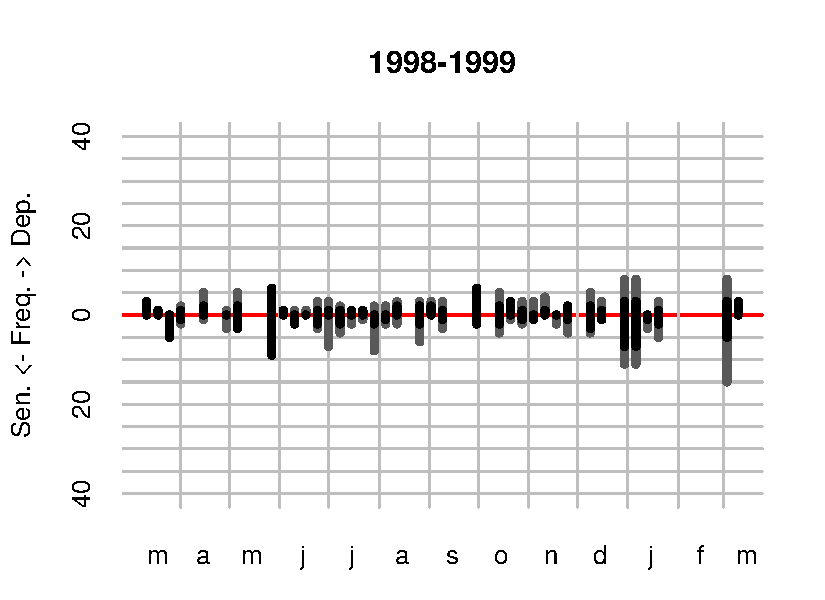
\includegraphics[width=.22\columnwidth]{../graphs/urgenciasHistog1998.pdf} &
    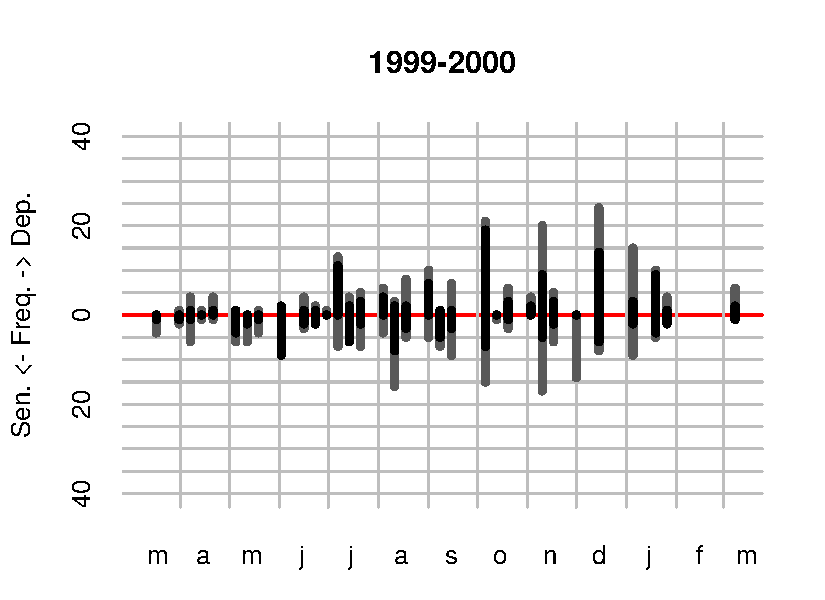
\includegraphics[width=.22\columnwidth]{../graphs/urgenciasHistog1999.pdf} &
    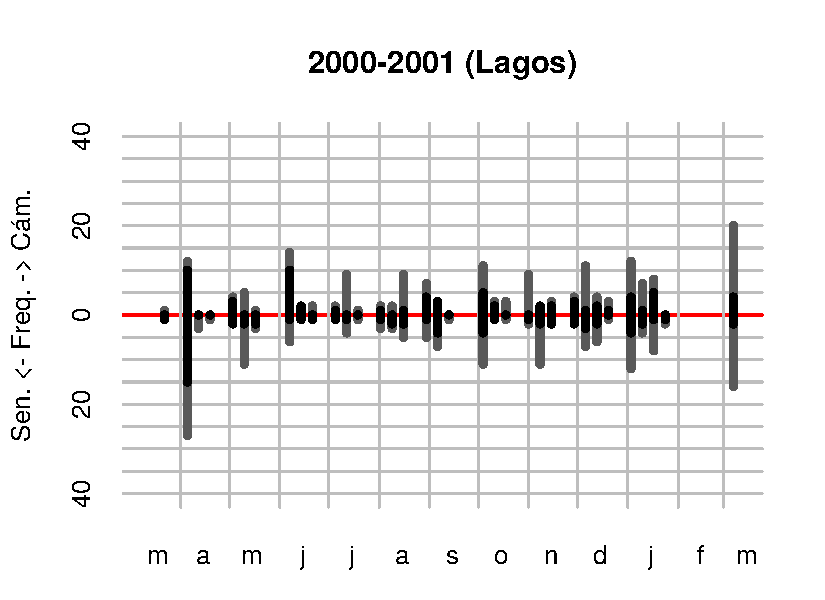
\includegraphics[width=.22\columnwidth]{../graphs/urgenciasHistog2000.pdf} &
    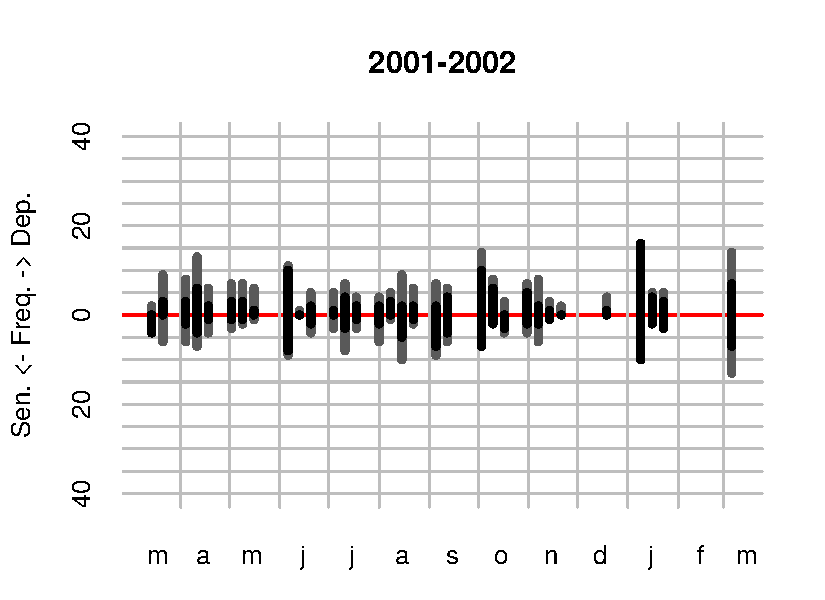
\includegraphics[width=.22\columnwidth]{../graphs/urgenciasHistog2001.pdf} \\
    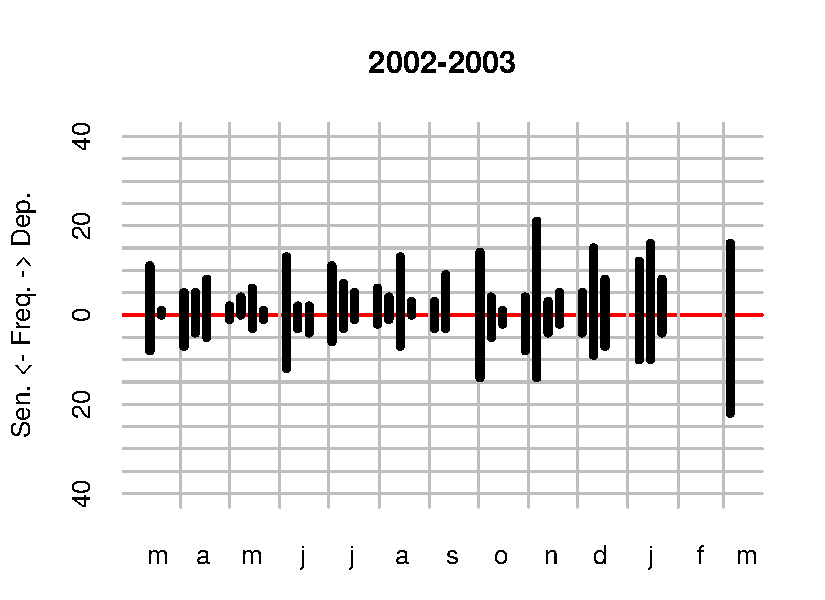
\includegraphics[width=.22\columnwidth]{../graphs/urgenciasHistog2002.pdf} &
    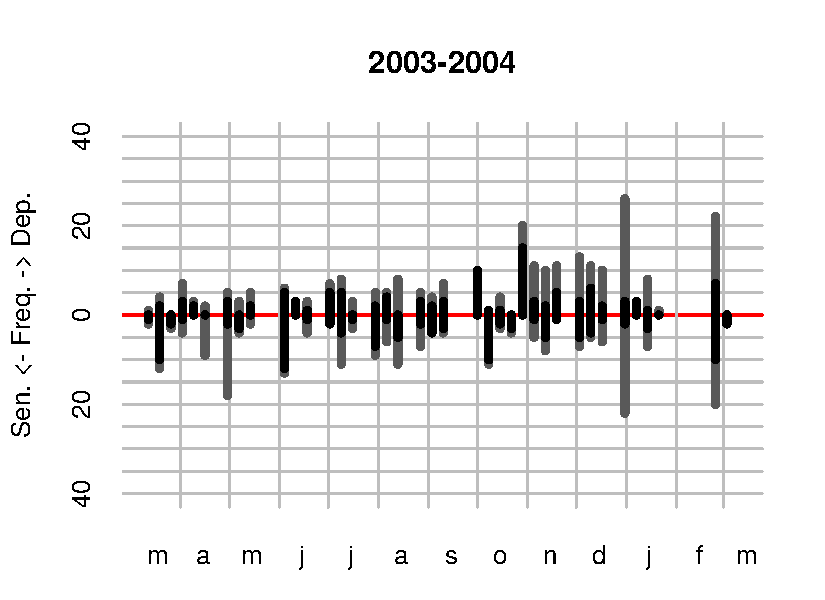
\includegraphics[width=.22\columnwidth]{../graphs/urgenciasHistog2003.pdf} &
    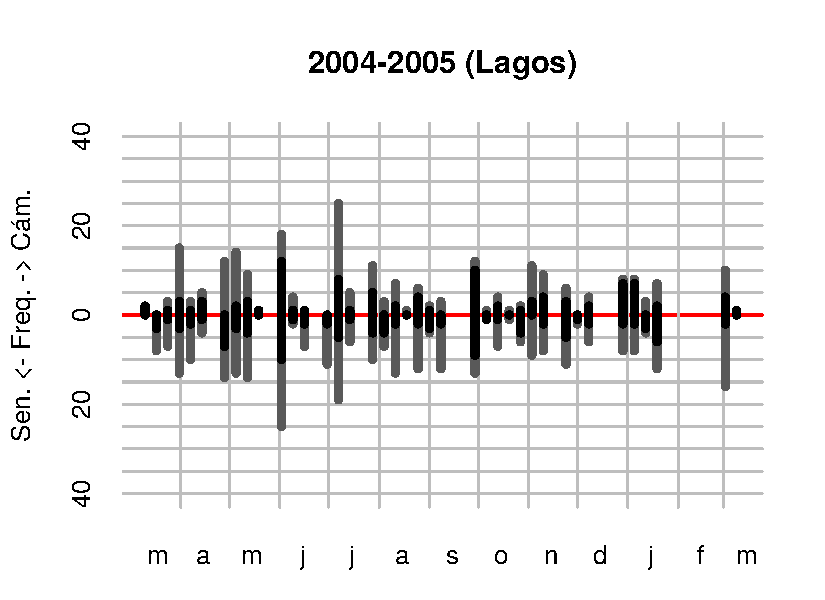
\includegraphics[width=.22\columnwidth]{../graphs/urgenciasHistog2004.pdf} &
    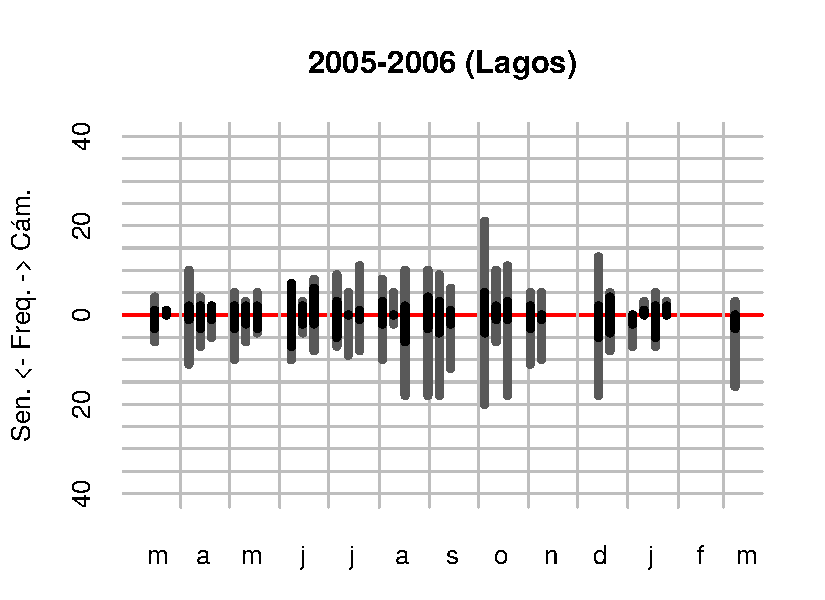
\includegraphics[width=.22\columnwidth]{../graphs/urgenciasHistog2005.pdf} \\
    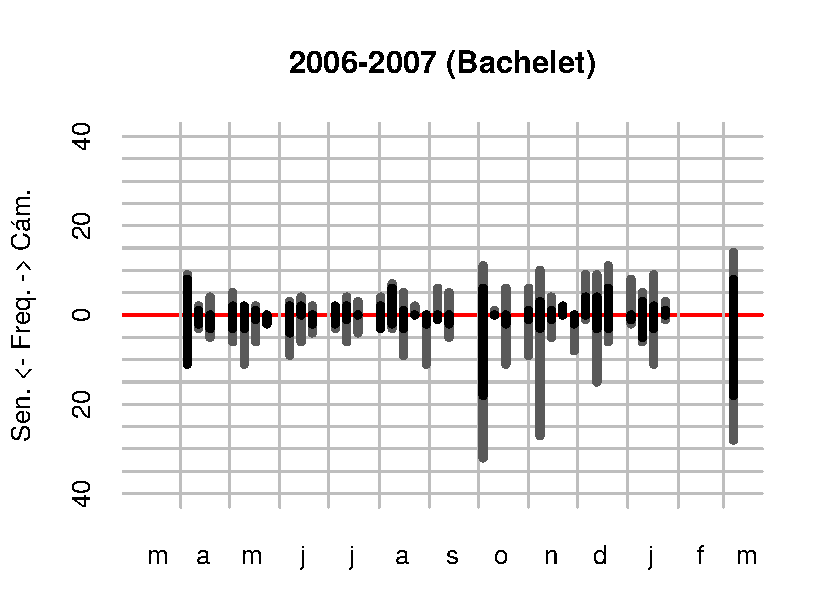
\includegraphics[width=.22\columnwidth]{../graphs/urgenciasHistog2006.pdf} &
    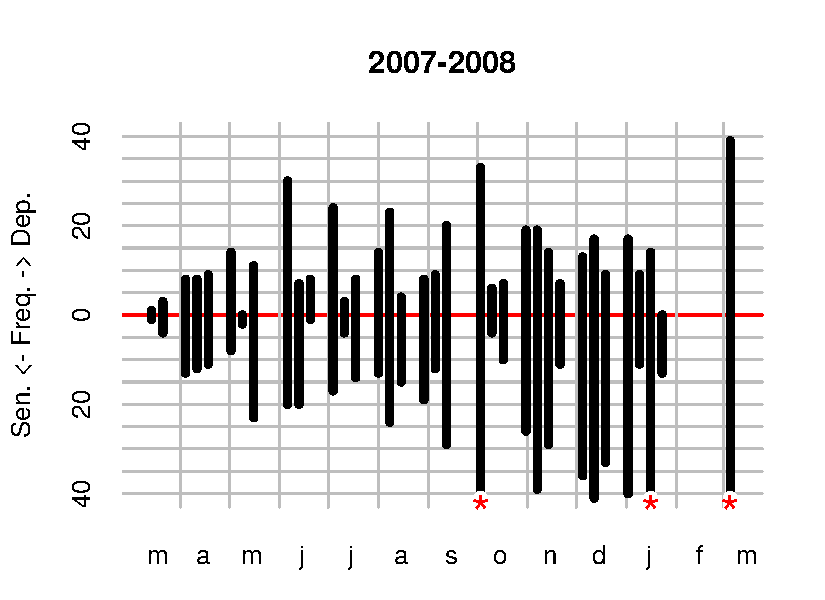
\includegraphics[width=.22\columnwidth]{../graphs/urgenciasHistog2007.pdf} &
    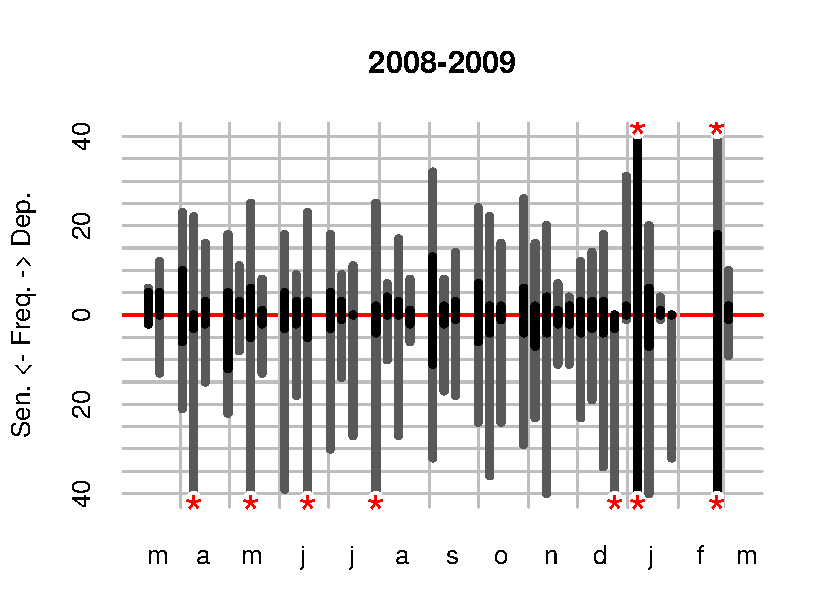
\includegraphics[width=.22\columnwidth]{../graphs/urgenciasHistog2008.pdf} &
    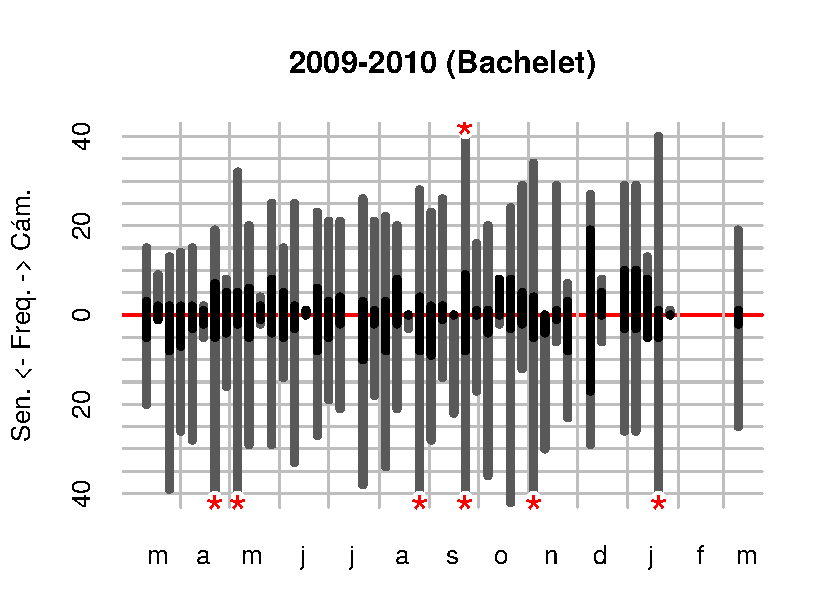
\includegraphics[width=.22\columnwidth]{../graphs/urgenciasHistog2009.pdf} \\
    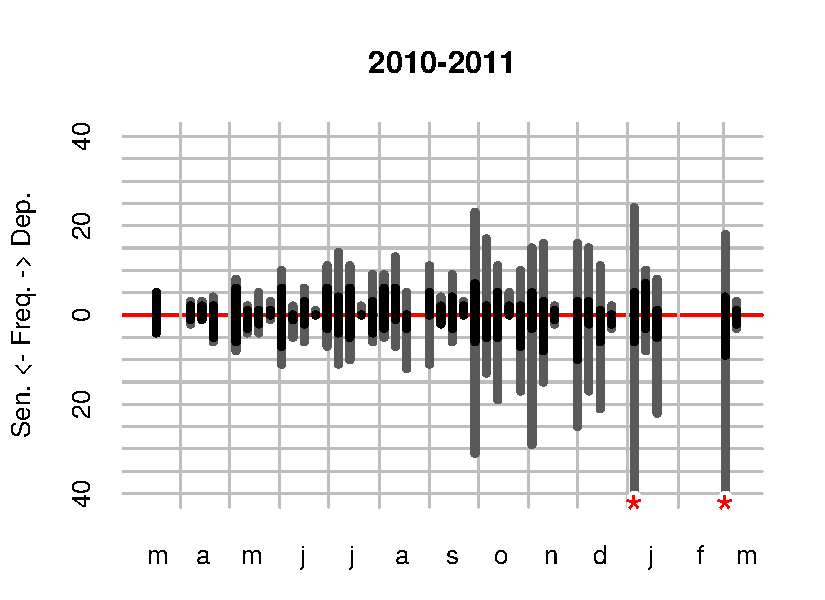
\includegraphics[width=.22\columnwidth]{../graphs/urgenciasHistog2010.pdf} &
    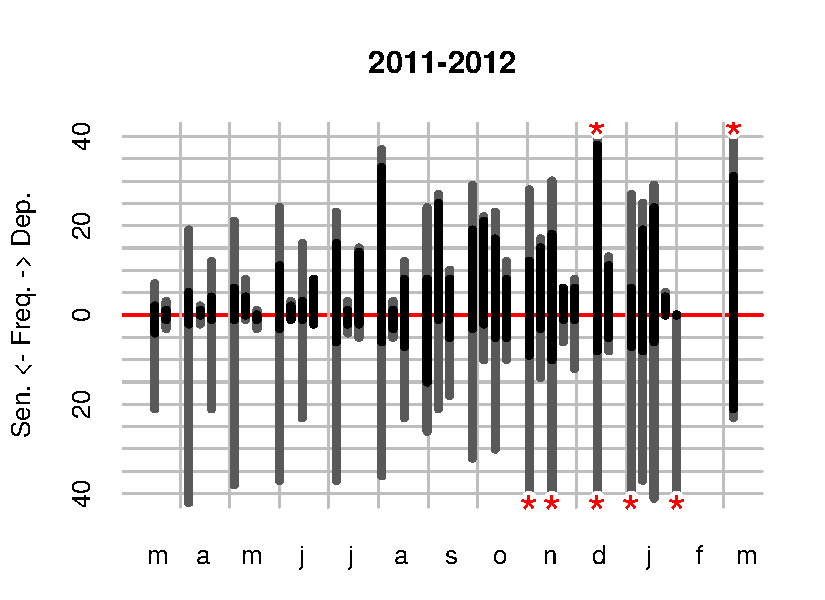
\includegraphics[width=.22\columnwidth]{../graphs/urgenciasHistog2011.pdf} &
    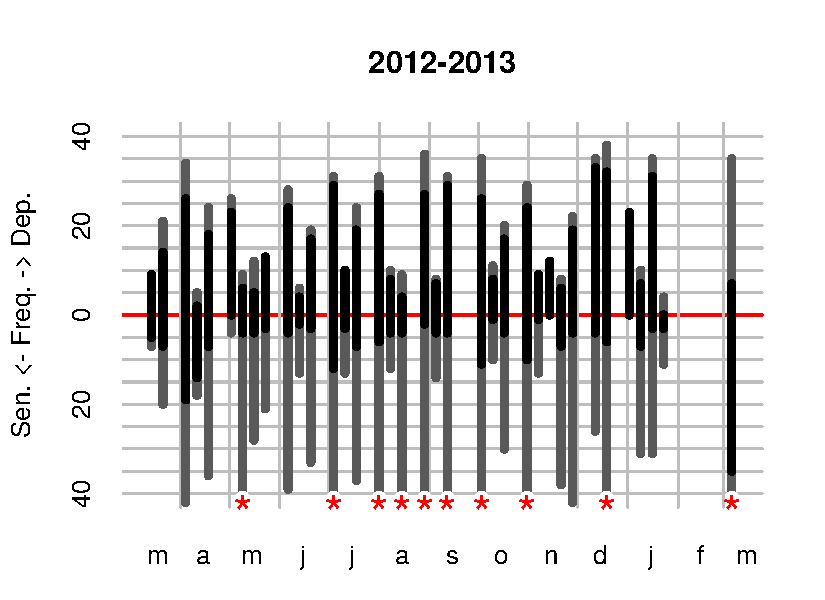
\includegraphics[width=.22\columnwidth]{../graphs/urgenciasHistog2012.pdf} &
    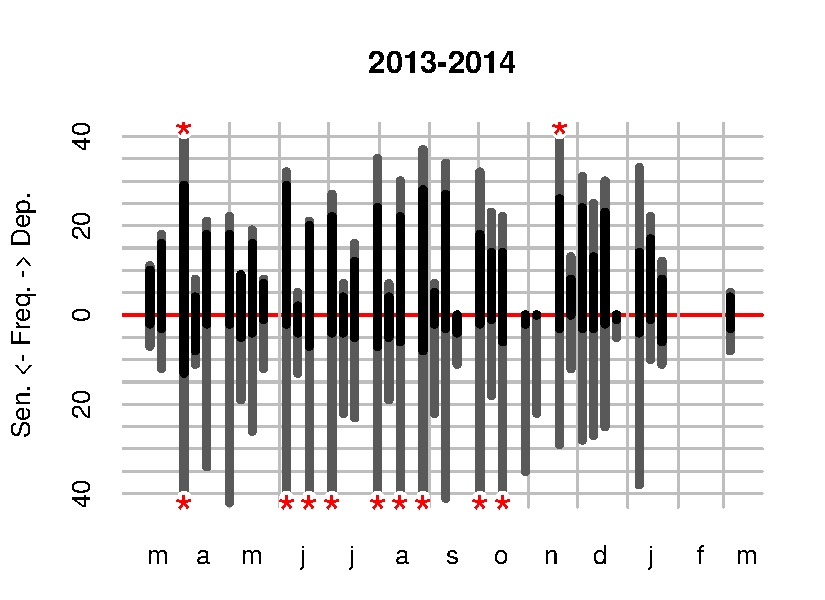
\includegraphics[width=.22\columnwidth]{../graphs/urgenciasHistog2013.pdf} \\
\end{tabular}
  \caption{Weekly urgencies by legislative year. Deputies histogram above, Senate below the zero line. Asterisk atop column indicates off-the-chart urgency message frequency. Source: prepared with data from the Chilean Congress.}\label{f:depvarHistog}
\end{center}
\end{figure}


There are detailed plots, keep only one year

% \begin{sidewaysfigure}
% \begin{center}
%     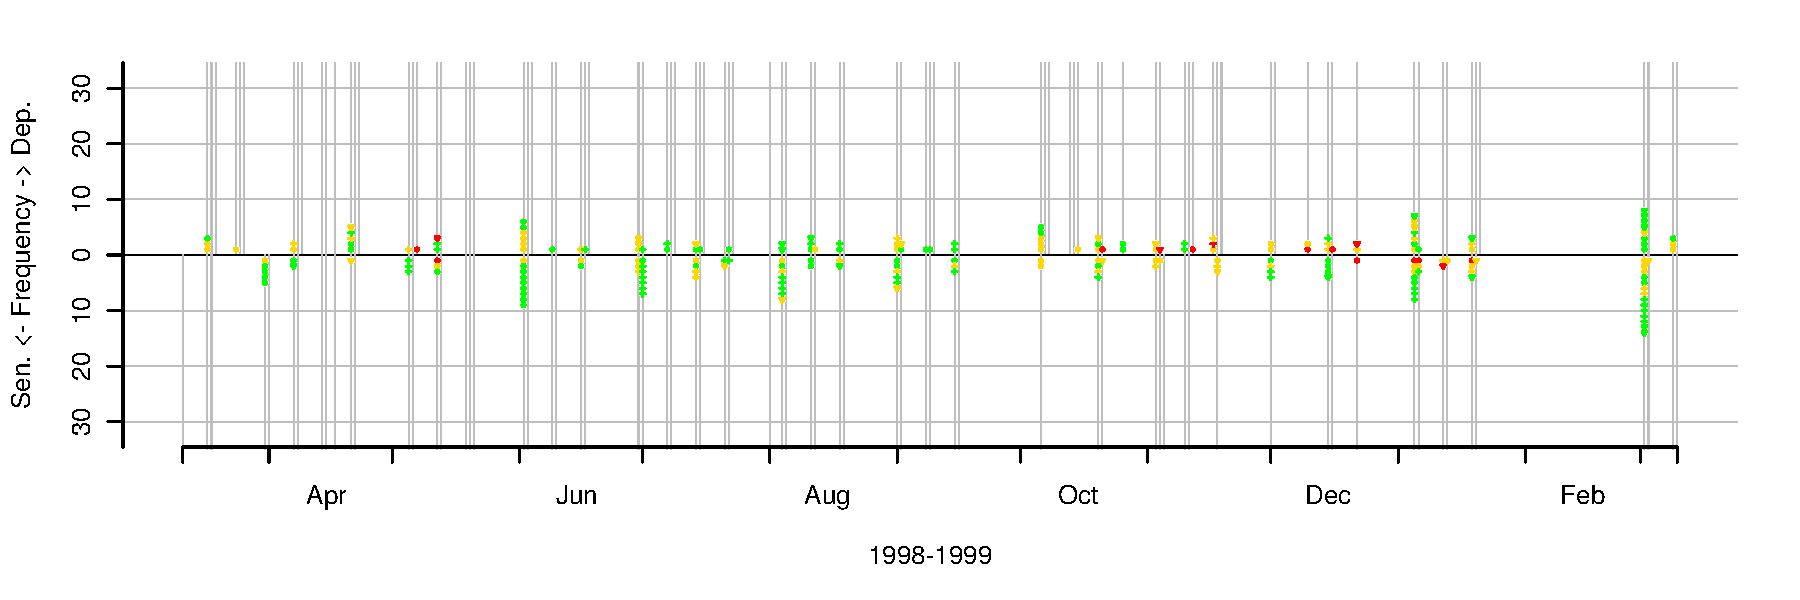
\includegraphics[width=\columnwidth]{../graphs/urgencias1998.pdf} \\
%     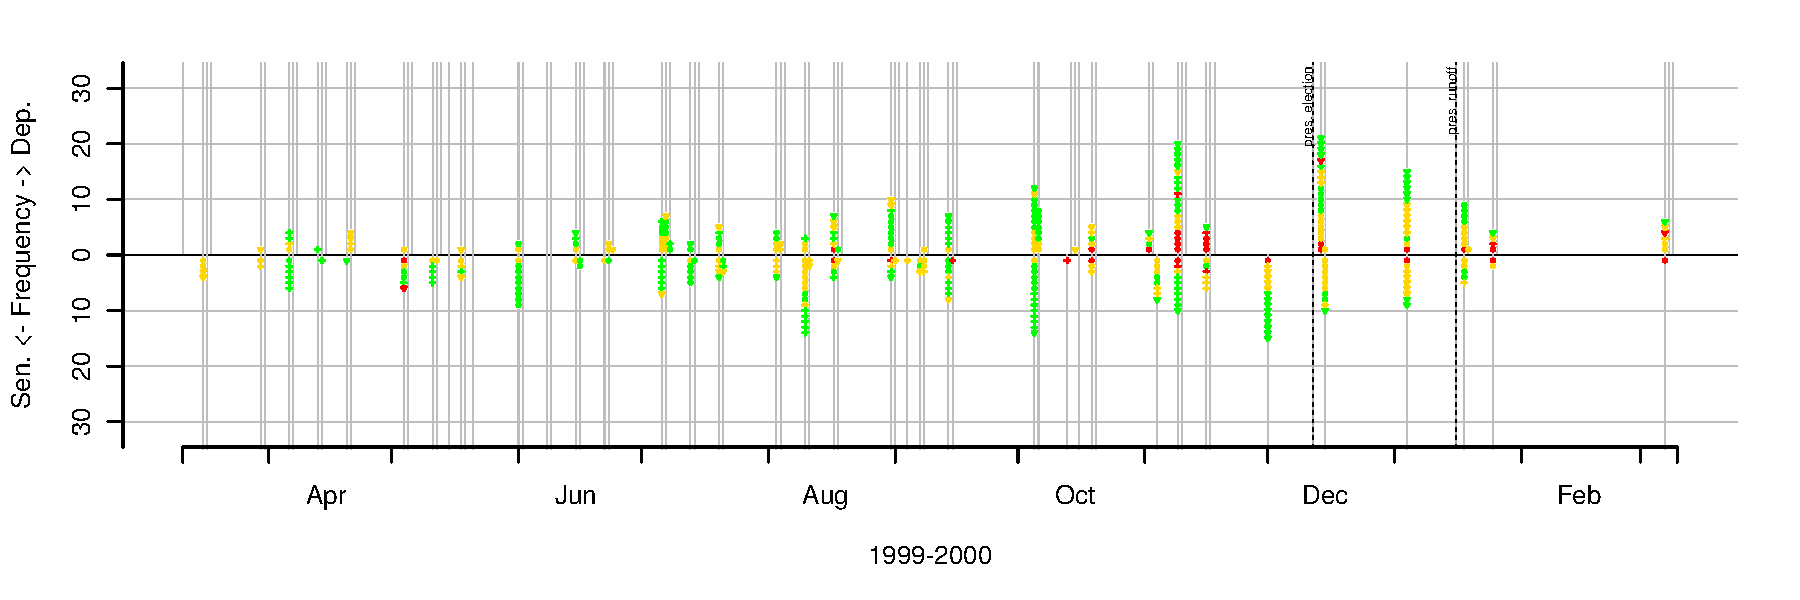
\includegraphics[width=\columnwidth]{../graphs/urgencias1999.pdf} 
%   \caption{Urgencies by legislative year. Deputies and Senate histograms above and below the zero line, respectively. Vertical grey lines indicate that a session took place. One point for each urgency message, a circle for a newly declared urgent bill, a plus sign for an urgent bill with new deadline, an inverted triangle for a retired urgency. Point color indicates the urgency deadline, red for 3/6 days, yellow for 10/15 days, green for 30 days. Parentheses atop columns indicate off-the-chart urgency message frequency.}\label{f:depvar}
% \end{center}
% \end{sidewaysfigure}

% \begin{sidewaysfigure}\ContinuedFloat
% \begin{center}
%     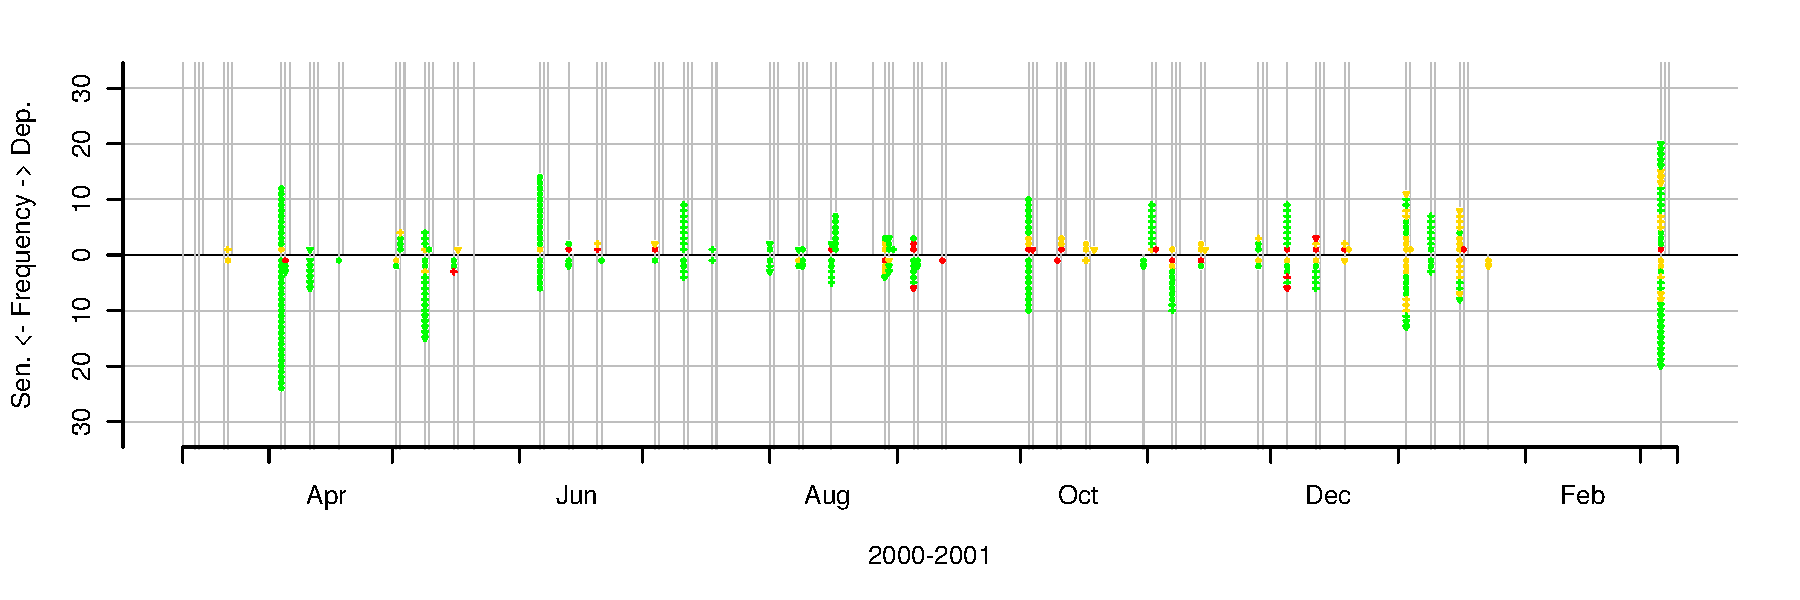
\includegraphics[width=\columnwidth]{../graphs/urgencias2000.pdf} \\
%     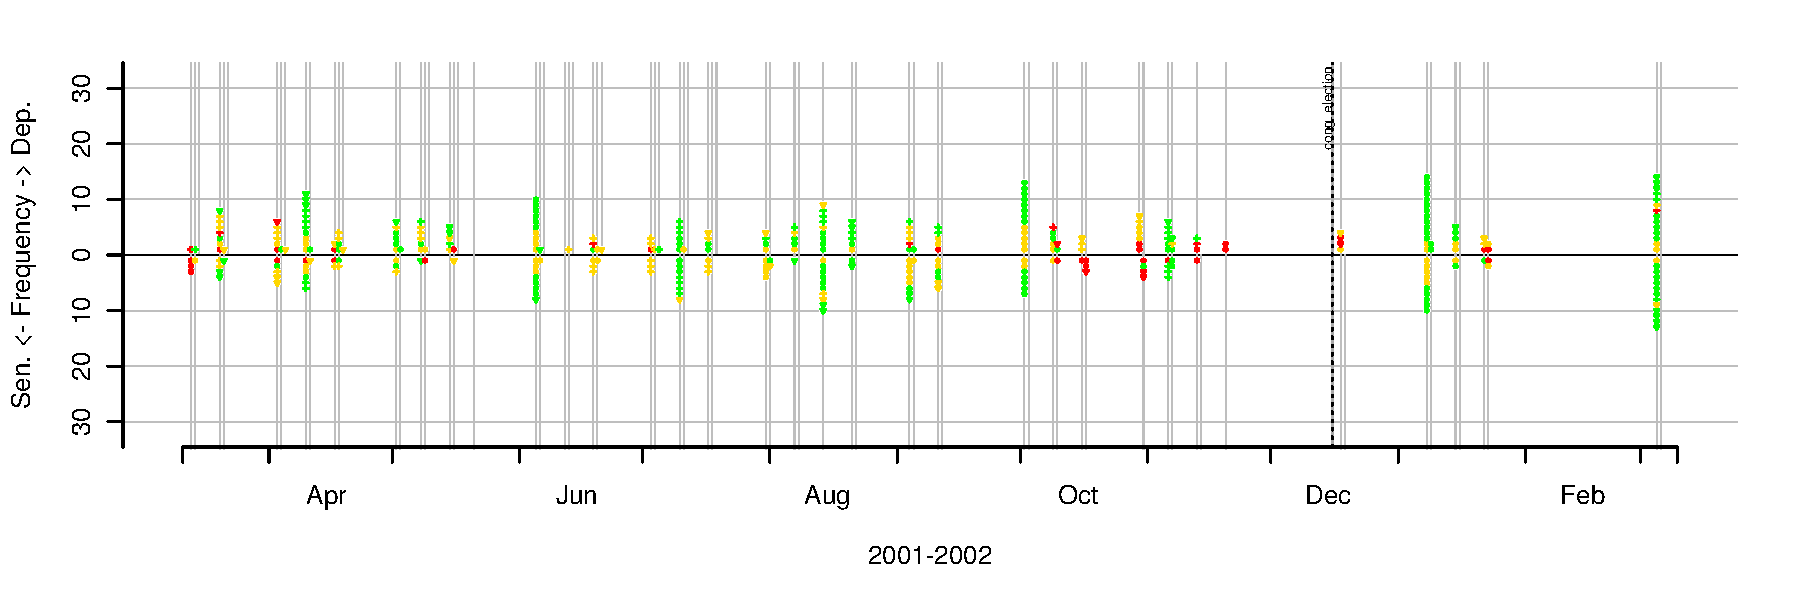
\includegraphics[width=\columnwidth]{../graphs/urgencias2001.pdf} 
%   \caption{Urgencies by legislative year (cont.)}\label{f:depvar}
% \end{center}
% \end{sidewaysfigure}

\begin{figure}
\begin{center}
    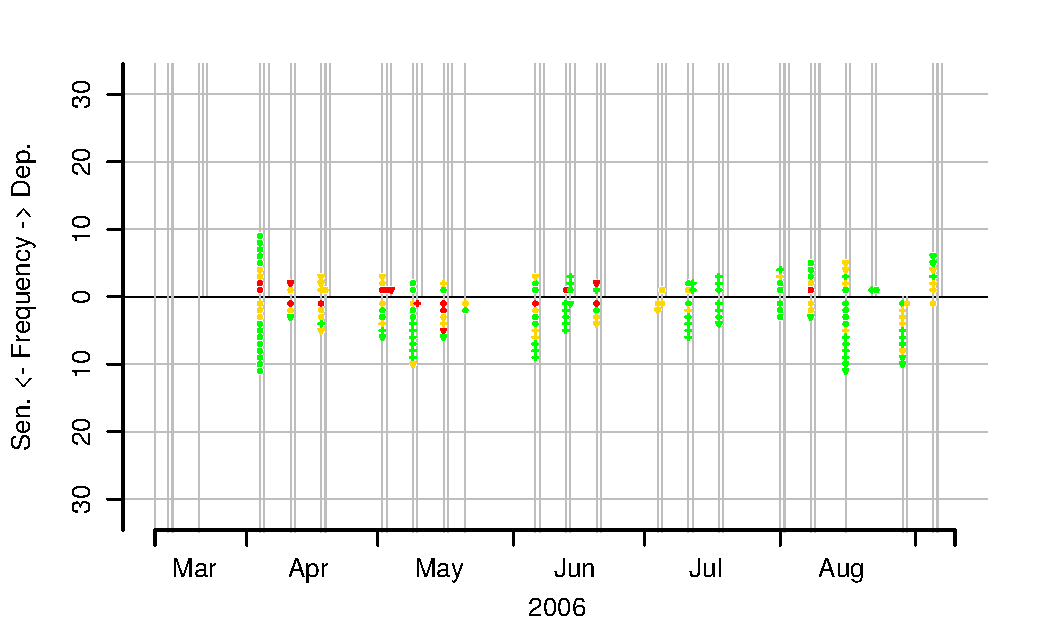
\includegraphics[width=\columnwidth]{../graphs/urgencias2006-1.pdf} \\
    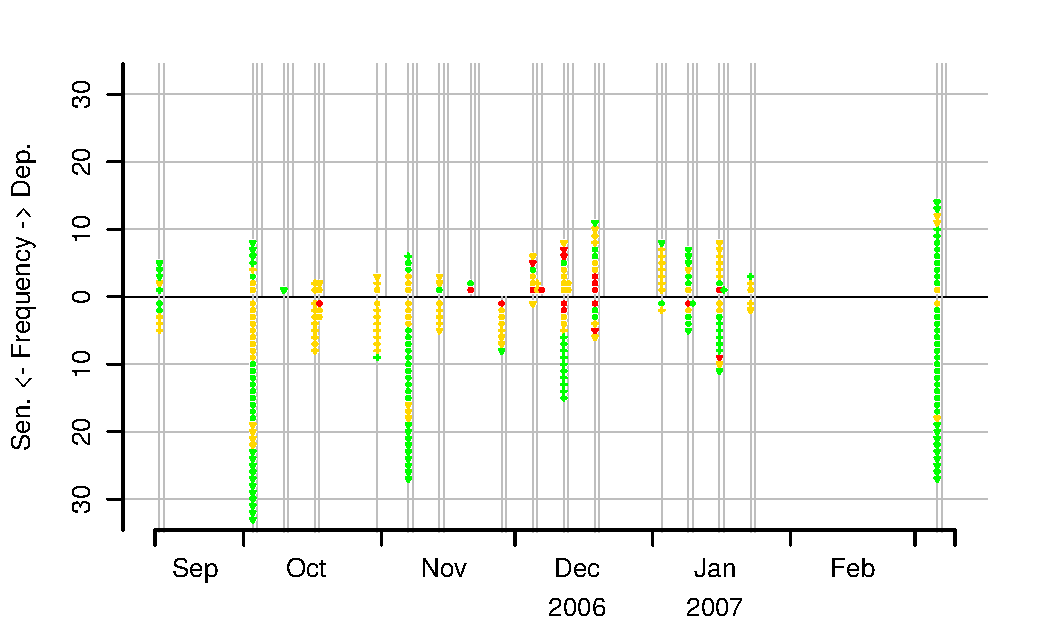
\includegraphics[width=\columnwidth]{../graphs/urgencias2006-2.pdf} 
  \caption{Urgencies in one legislative year. Deputies and Senate data above and below the zero line, respectively. Vertical grey lines indicate that a session took place. One point for each urgency message, a circle for a newly declared urgent bill, a plus sign for an urgent bill with new deadline, an inverted triangle for a retired urgency. Point color indicates the urgency deadline, red for 3/6 days, yellow for 10/15 days, green for 30 days. Parentheses atop columns indicate off-the-chart urgency message frequency.}\label{f:depvar}
\end{center}
\end{figure}





 



\section{Committee reporting}

Committee reporting is one step of the legislative process where the effects of urgency usage can be gauged. Unless the floor votes an exception unanimously, every bill in Chile is referred to a standing or special committee upon first introduction to each chamber. In this prefloor stage, a committee chooses to schedule or not a bill for discussion and hearings towards drafting a proposal for the plenary. Discretion to prioritize legislation could in principle translate into negative or gatekeeping power, and bill drafting into positive power---possibly turning standing committees into formidable actors in their jurisdiction \citep{cox.mccubbins.1993,fenno.1973,shepsle.weingast.1987}. No explicit discharge procedure exists in the Reglamento, but presumably is the same---unanimous consent---to except a bill from referral to committee. 

The Hacienda (Finance) committee has special status in the committee system and deserves attention. It stands apart from other committees because it has jurisdiction over all bills authorizing spending in any domain (multiple referrals are common, how many?). Bills with authorizations \emph{must} be referred to Hacienda, and the unanimous exception is inapplicable. Hacienda committee members, working along with Finance Ministry staff \citep{aleman.navia.UrgChi.2009}, may or may not appropriate funds from the budget when reporting the bill to the floor. Not unlike the Appropriations committee in the U.S.\ House, Hacienda has the status of a control committee, a key link towards agenda control \citep{kiewiet.mccubbins.1991}. 

Yet the urgency authority can be suspected of undermining the gatekeeping potential of committees. Unless urgency messages can be ignored with ease, committee inaction on undesirable but urgent legislation becomes impossible. 

There are measurement and methodological challenges to study effects of urgency authority usage. Selection problems make gauging effects on the likelihood of bill passage, for example, difficult. Whether or not they lead to vote exchange, for example, seems to require data unavailable so far. But committee reports offer an opportunity---observable in bill histories, might help detect if urgencies are heeded in Congress. 

Discuss failure to observe a report after an urgency: should not immediately conclude that urgencies are dead weight. Bill may have already been reported and be stuck in bottleneck down the stream. But unless there is a reason to suspect that most or many  urgency messages arrive after the committee has reported---there is no a priori reason to expect this---a fair number of messages should be followed by a report. And the wait should bear relation to the degree of the urgency. 

Hypothesis 1: urgency message is followed by increased committee report activity in the chamber. 

Hypothesis 2: bills referred to Hacienda declared urgent followed by more reports from that committee.

Hypothesis 3: increased report activity after urgencies happens within the deadline established by the urgency message.


\begin{table}
\begin{center}
\begin{tabular}{lrrr}
                    &  \mc{3}{c}{Report observed within deadline} \\
Urgency message     &  ~~~~~~\% yes  &  ~~~~~~\% no   &  N     \\ \hline
Act now             &  63      &  37      &  475   \\
2-week notice       &  27      &  73      &  2192  \\
4-week notice       &  25      &  75      &  1678  \\
Deadline shortened  &  41      &  59      &  241   \\
Deadline extended   &  23      &  77      &  3454  \\
Withdrawn           &  6       &  94      &  211   \\ \hline
All                 &  27      &  73      &  8251  \\
\end{tabular}
\caption{Urgency messages and committee reports within deadline, 2006--2014}
\end{center}
\end{table}

Weekly aggregates were computed from the data. The dependent variable is the number of bills reported by some C\'amara committee any given week. Weeks when the C\'amara did not meet were dropped, adding any bill reported to the closest next week with a session.\footnote{Bill histories date reports when officially received (\emph{cuenta}), but some cases have prior mention to the report's finalization, which the algorithm incorrectly coded as the date. The same is true for weekly urgency messages, with figures for weeks with diputados not meeting corrected likewise.} Two figures were produced for analysis: weekly Hacienda committee reports, and weekly reports from any committee. The Hacienda aggregate seems preferable, letting analysis search for correlation with urgency messages explicitly targeting bills that were referred to that committee at some point. The total aggregate offers less control, but a more comprehensive picture. The average week in the 2006--2010 period had reports...

Dependent variable is limited (a count, non-negative integer). Negative binomial regression for analysis. Included in the right side are weekly urgency messages. Aggregates distinguish different urgency messages: the number of act-now, 2-week, and 4-week notices, deadlines shortened, extended, and withdrawals. If some bill is given an act now message, an effect should be observed almost immediately, the current week or the next at most. But other urgency message effects, if any, should not necessarily be so immediate---legislators must react, and that takes time. In order to capture this, weekly lags of the regressors were included in the analysis. 


%%%% NegBin Regressions from chilBill.r 
% 1Regression of Hda Reports to Exec bills on Urgencies to Exec bills ref to Hda  DIP
% (Intercept)   . 
% nNow          ++ nNowl1        +  nNowl2        --
%                  n2wkl1        ++ n2wkl2        .   n2wkl3        --
%                                   n4wkl2        .   n4wkl3        ++   n4wkl4        ++
% nShorten       . nShortenl1    ++ nShortenl2    . 
%  dterm         . 
%  dleg10        --
% 
% 2Regression of All Reports to Exec bills on Urgencies to Exec bills ref anywhere  DIP
% (Intercept)   ++
% nNow          ++ nNowl1        ++ nNowl2        --
%                  n2wkl1        +  n2wkl2        ++ n2wkl3        . 
%                                   n4wkl2        .  n4wkl3        .  n4wkl4        . 
% nShorten      .  nShortenl1    .  nShortenl2    . 
% dterm         . 
% dleg10        --
% 
% 3Regression of Hda Reports to Leg bills on Urgencies to Exec bills ref to Hda  DIP
% (Intercept)   --
% nNow          .  nNowl1        ++
% n2wk          ++ n2wkl1        -  n2wkl2        ++
% 
%                  nShortenl1    . 
% dterm         . 
% dleg10        --
% 
% 4Regression of All Reports to Leg bills on Urgencies to Exec bills ref anywhere  DIP
% > + + + +  
%            coef
% (Intercept)   ++
% nNow          . nNowl1        . 
% n2wk          + 
% n2wkl1        . n2wkl2        . n2wkl3        . n2wkl4        --
% n4wkl1        . n4wkl2        . n4wkl3        . n4wkl4        ++
% nShorten      . nShortenl1    . nShortenl2    . 
% dterm         . 
% dleg10        . 
% 
% 5Regression of Hda Reports to Leg bills on Urgencies to Leg bills ref Hda Comm  DIP
%            coef
% (Intercept)   --
% nNow          ++ nNowl1        ++
%                  n2wkl1        .  n2wkl2        ++ n2wkl3        ++
%                                   n4wkl2        .  n4wkl3        .  n4wkl4        . 
% dterm         . 
% dleg10        --
\begin{table}
\begin{tabular}{l|ccccc|ccccc}
                 & \mc{10}{c}{Effect on committee reports ($t=0$ is current week)}                                      \\
%                 &   \mc{10}{c}{Dependent variable:} \\ 
                 & \mc{5}{c|}{DV = exec.~bill reports}      & \mc{5}{c}{DV = member bill reports}                      \\
Type             & $t=0$    & 1        & 2       & 3       & 4         & $t=0$    & 1          & 2         & 3          & 4          \\ \hline
\mc{11}{l}{\emph{IV: urgencies targeting executive bills referred to Hacienda committee}}  \\
                 &                    \mc{5}{c|}{(a)}                   &                       \mc{5}{c}{(b)}                         \\ 
Act Now          &   $++$   &  $+$     &   $--$  &         &           &          &  $++$      &           &            &            \\
2-week notice    &          &  $++$    &         &    $--$ &           &     $++$ &  $-$       &  $++$     &            &            \\
4-week notice    &          &          &         &    $++$ &      $++$ &          &            &           &            &            \\
Shorten deadline &          &  $++$    &         &         &           &          &            &           &            &            \\ \hdashline
\mc{11}{l}{\emph{IV: urgencies targeting member~bills referred to Hacienda committee}}    \\
                 &                    \mc{5}{c|}{(c)}                   &                       \mc{5}{c}{(d)}                         \\ 
Act Now          &          &          &         &         &           &     $++$ &  $++$      &           &            &            \\
2-week notice    &          & \mc{3}{c}{\footnotesize{(not estimated)}} &           &          &            &  $++$     &      $++$  &            \\ 
4-week notice    &          &          &         &         &           &          &            &           &            &            \\  
Shorten deadline &          &          &         &         &           &          &            &           &            &            \\ \hdashline
\mc{11}{l}{\emph{IV: urgencies targeting any executive bill}}  \\
                 &                    \mc{5}{c|}{(e)}                   &                       \mc{5}{c}{(f)}                         \\ 
Act Now          &   $++$   &  $++$    &   $--$  &         &           &          &            &           &            &            \\
2-week notice    &          &  $+$     &   $++$  &         &           &     $+$  &            &           &            &      $--$  \\
4-week notice    &          &          &         &         &           &          &            &           &            &      $++$  \\
Shorten deadline &          &          &         &         &           &          &            &           &            &            \\ \hline
\mc{11}{l}{\footnotesize{$++,--: p<.05$; $+,-: p<.1$ (one-tailed tests)}}                                                            \\
\end{tabular}
\caption{Effect of weekly urgency messages on committee reports, C\'amara de Diputados 2006--2014. Entries report signs and significance (one-tailed) of regression coefficients. Negative binomial method of estimation, with fixed Legislature effects (see text).}\label{t:negbin}
\end{table}

Table \ref{t:negbin} offers a synthetic view of results, showing the sign and significance of key coefficients only---urgencies observed and lags. The form of the general model estimated is $\text{nReports}_t = \beta_0 + \beta_1 \text{nUrgencies}_t + \beta_2 \text{nUrgencies}_{t-1} + ...$, where $t$ is the current week, $t-1$ the week before, and so forth up to four lags. The right side makes a distinction of the number of weekly Act-now, 2-week, and 4-week notices. It also controls for (but the table does not report) the percentage of the current legislative year remaining and a dummy distinguising the 2010--2014 legislature (from the 2006--2010 baseline). 

Models for weekly reports to executive (models a, c, e) and to MC bills (model b, d, f) were estimated separately. Effects of aiming the urgency authority at different subsets of projects were investigated. So model (a) goes in search of how the number of weekly urgencies to executive bills referred to Hacienda affect weekly reports by that committee of executive bills. Model (b) does the same number of weekly urgencies affect Hacienda committee reports of MC bills. 

Results are interesting. Model (a) should have positive effects, and it mostly does. Act-now and shorten dealine messages associated with a surge in reports the current week or next at most. Other urgency messages produce a surge later, as expected. A significant drop in reporting activity observed after the deadline---Hacienda committee changes focus from executive bills to other business?  

Model (b) should have negative effects (the effect of declaring executive bills urgent on reports of MC bills in the Hacienda committee). The opposite is observed for act-now and 2-week notices: rather than pushing pending business due to a shock in the agenda, the Hacienda committee appears to hasten their report.  

Model (d) similar to (a) with focus on MC bills in Hacienda, should have positive effects, as it does. Similar results: urgency messages followed by surge in reporting activity. No slump afterwards. No effect of 4-week deadlines nor shorter deadlines here. 

Models (e) and (f) reveal the searching for chamber wide effects at one is harder, especially for MC bills. But patterns for executive bills match those of teh Hacienda committee.  


\section{Determinants of urgency messages}

Here the unit is the individual bill. The dependent variable dichotomous: whether or not the bill received at least one urgency message at some point. Controls for bill authorship: bills by any member of Congress; bills by opposition members of Congress, or by members of the presidential coalition, or co-sponsored by opposition and presidential coalition members. The omitted category are executive bills. Also controls for bills referred to Hacienda (dummy), whether the president had majority status in the Senate; if the bill was introduced in the Senate; the \% presidential term remaining when the bill was initiated; and the \% legislative year remaining. 

Logit method of estimation. Goodness of fit ok (89 percent correct prediction). Should run exec and MC separate. 


% Table created by stargazer v.5.1 by Marek Hlavac, Harvard University. E-mail: hlavac at fas.harvard.edu
% Date and time: Mon, Feb 02, 2015 - 05:55:22 PM
% Requires LaTeX packages: dcolumn 
\begin{table}[!htbp] \centering 
\begin{tabular}{@{\extracolsep{5pt}}lD{.}{.}{-3} D{.}{.}{-3} } 
\\[-1.8ex]\hline 
\hline \\[-1.8ex] 
 & \multicolumn{2}{c}{\textit{Dependent variable:}} \\ 
\cline{2-3} 
\\[-1.8ex] & \multicolumn{2}{c}{Any urgency} \\ 
\\[-1.8ex] & \multicolumn{1}{c}{(1)} & \multicolumn{1}{c}{(2)}\\ 
\hline \\[-1.8ex] 
 MC bill & -2.978^{***} &  \\ 
  & (0.090) &  \\ 
  & & \\ 
 MC bill, opp.-sponsored &  & -3.597^{***} \\ 
  &  & (0.137) \\ 
  & & \\ 
 MC bill, mix.-sponsored &  & -2.517^{***} \\ 
  &  & (0.114) \\ 
  & & \\ 
 MC bill, pres. coal.-sp. &  & -2.969^{***} \\ 
  &  & (0.126) \\ 
  & & \\ 
 Hacienda & 1.761^{***} & 1.782^{***} \\ 
  & (0.111) & (0.111) \\ 
  & & \\ 
 Senate majority & -0.304^{***} & -0.302^{***} \\ 
  & (0.086) & (0.086) \\ 
  & & \\ 
 Introduced Senate & 0.184^{*} & 0.415^{***} \\ 
  & (0.096) & (0.111) \\ 
  & & \\ 
 Pres.~term remaining & 0.004^{***} & 0.004^{***} \\ 
  & (0.002) & (0.002) \\ 
  & & \\ 
 Year remaining  & 0.003 & 0.003^{*} \\ 
  & (0.002) & (0.002) \\ 
  & & \\ 
 Constant & -0.047 & -0.113 \\ 
  & (0.140) & (0.141) \\ 
  & & \\ 
\hline \\[-1.8ex] 
Observations & \multicolumn{1}{c}{6,987} & \multicolumn{1}{c}{6,987} \\ 
Log Likelihood & \multicolumn{1}{c}{$-2,057$} & \multicolumn{1}{c}{$-2,029$} \\ 
\% predicted correctly & \multicolumn{1}{c}{89} & \multicolumn{1}{c}{89} \\ 
\hline 
\hline \\[-1.8ex] 
\textit{Note:}  & \multicolumn{2}{r}{$^{*}$p$<$0.1; $^{**}$p$<$0.05; $^{***}$p$<$0.01} \\ 
\end{tabular} 
  \caption{Regression results} \label{} 
\end{table} 




% Table created by stargazer v.5.1 by Marek Hlavac, Harvard University. E-mail: hlavac at fas.harvard.edu
% Date and time: Thu, Feb 05, 2015 - 09:04:18 PM
% Requires LaTeX packages: dcolumn 
\begin{table}[!htbp] \centering 
  \caption{Regression results} 
  \label{} 
\begin{tabular}{@{\extracolsep{5pt}}lD{.}{.}{-3} D{.}{.}{-3} D{.}{.}{-3} } 
\\[-1.8ex]\hline 
\hline \\[-1.8ex] 
 & \multicolumn{3}{c}{\textit{Dependent variable:}} \\ 
\cline{2-4} 
\\[-1.8ex] & \multicolumn{1}{c}{Act now} & \multicolumn{1}{c}{2-week} & \multicolumn{1}{c}{4-week} \\ 
\\[-1.8ex] & \multicolumn{1}{c}{(3)} & \multicolumn{1}{c}{(4)} & \multicolumn{1}{c}{(5)}\\ 
\hline \\[-1.8ex] 
 MC bill & -3.469^{***} & -3.442^{***} & -2.843^{***} \\ 
  & (0.298) & (0.180) & (0.151) \\ 
  & & & \\ 
 MC bill, opp.-sponsored & -2.141^{***} & -2.267^{***} & -1.863^{***} \\ 
  & (0.216) & (0.141) & (0.126) \\ 
  & & & \\ 
 MC bill, mix.-sponsored & -2.403^{***} & -2.553^{***} & -2.251^{***} \\ 
  & (0.215) & (0.147) & (0.139) \\ 
  & & & \\ 
 MC bill, pres. coal.-sp. & 1.451^{***} & 1.290^{***} & 0.759^{***} \\ 
  & (0.129) & (0.105) & (0.103) \\ 
  & & & \\ 
 Hacienda & -0.288^{**} & -0.397^{***} & 0.037 \\ 
  & (0.114) & (0.092) & (0.087) \\ 
  & & & \\ 
 Senate majority & 0.526^{***} & 0.413^{***} & 0.199^{*} \\ 
  & (0.146) & (0.119) & (0.111) \\ 
  & & & \\ 
 Introduced Senate & 0.002 & 0.003^{*} & 0.004^{**} \\ 
  & (0.002) & (0.002) & (0.002) \\ 
  & & & \\ 
 Pres.~term remaining & 0.002 & 0.003^{**} & 0.003 \\ 
  & (0.002) & (0.002) & (0.002) \\ 
  & & & \\ 
 Year remaining & -1.990^{***} & -0.912^{***} & -1.167^{***} \\ 
  & (0.192) & (0.151) & (0.145) \\ 
  & & & \\ 
\hline \\[-1.8ex] 
Observations & \multicolumn{1}{c}{6,987} & \multicolumn{1}{c}{6,987} & \multicolumn{1}{c}{6,987} \\ 
Log Likelihood & \multicolumn{1}{c}{-1,132} & \multicolumn{1}{c}{-1,734} & \multicolumn{1}{c}{-1,980} \\ 
\% predicted correctly & \multicolumn{1}{c}{81} & \multicolumn{1}{c}{88} & \multicolumn{1}{c}{83} \\ 
\hline 
\hline \\[-1.8ex] 
\textit{Note:}  & \multicolumn{3}{r}{$^{*}$p$<$0.1; $^{**}$p$<$0.05; $^{***}$p$<$0.01} \\ 
\end{tabular} 
\end{table} 



\section{Extra material}


\begin{figure}
\begin{center}
    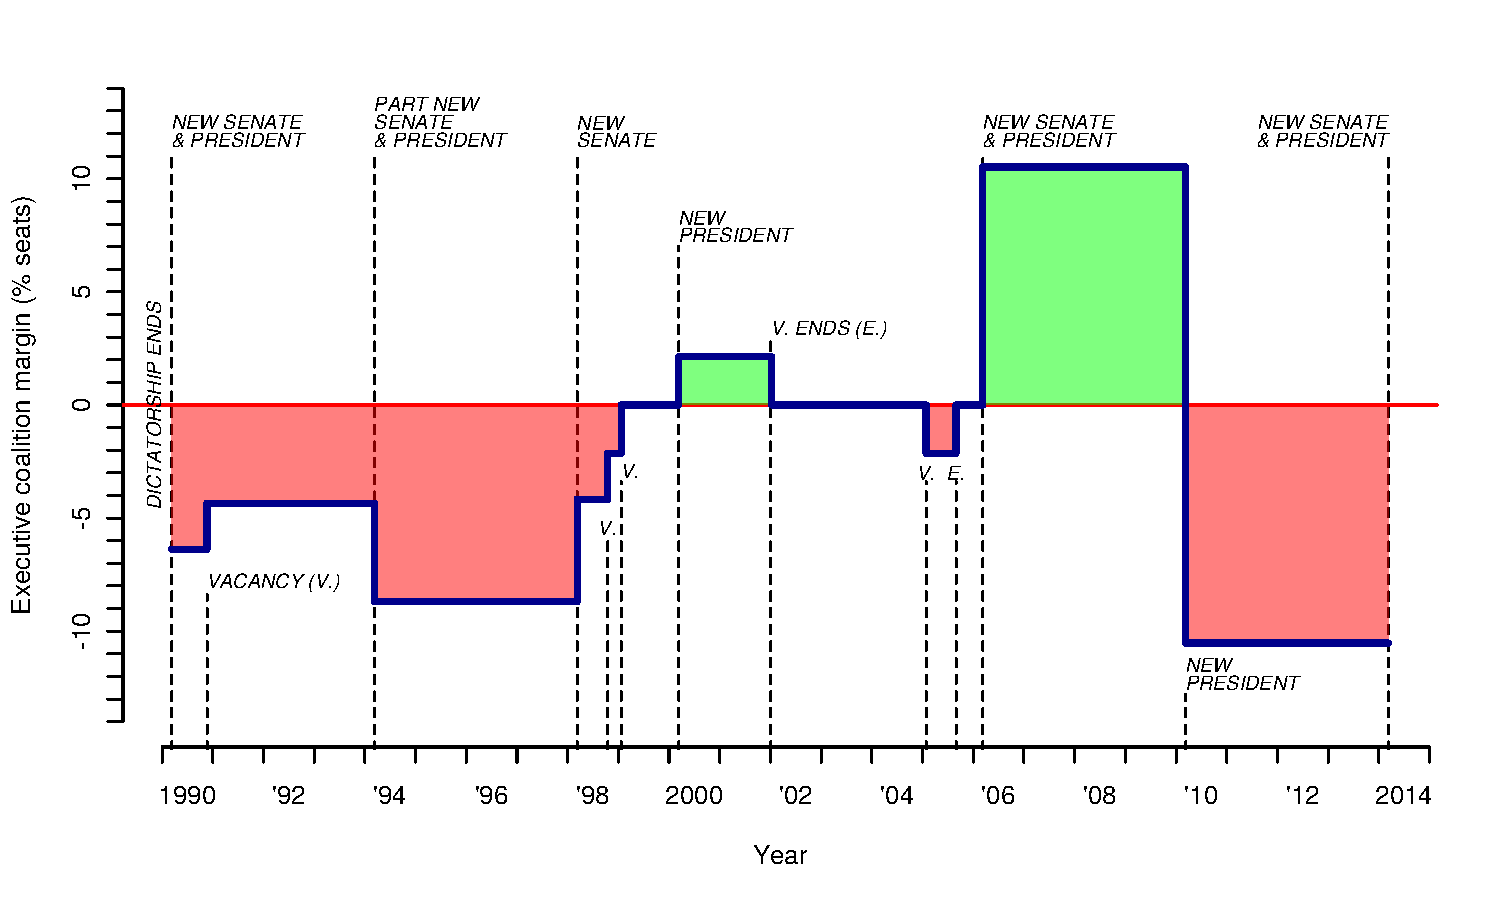
\includegraphics[width=\columnwidth]{../graphs/senChile.pdf}
  \caption{The Conservative chamber. The blue, crenellated line reports, longitudinally, the percentage of Senate seats controlled by the president's coalition minus the percentage controlled by the opposition. Totals include 38 elected senators and, up to 2006, 9 appointed senators and two or fewer senators for life. Vacancies, if any, are excluded; see text for details. The Senate renews in full every eight years, and was partially renewed in 1994. Vacancies reported: Ruiz Danyau, Air Force appointee, died in office 11/1990; Pinochet detained in London 10/1998; Errázuriz stripped of immunity 1/1999 (resinstated 1/2002); Lavandero stripped of immunity 1/2005 (replaced upon conviction 8/2005). }\label{f:senChile}
\end{center}
\end{figure}





% % \begin{tabular}{lrrrrrr}
% %                                   &  \mc{2}{c}{passed}    &  \mc{2}{c}{not}     &  \mc{2}{c}{all}      \\    
% % Bills with urgency in             &  N     &  \%          &  N     &  \%        &  N     &  \%         \\ \hline
% % $1^{st}$ chamber only              &   122  &  \emph{32}   &   259  &  \emph{68} &   381  &  \emph{100} \\
% % $2^{nd}$ chamber only              &   129  &  \emph{68}   &    62  &  \emph{32} &   191  &  \emph{100} \\
% % conference only                   &    27  &  \emph{82}   &     6  &  \emph{18} &    33  &  \emph{100} \\
% % $1^{st}$ and $2^{nd}$               &   363  &  \emph{81}   &    87  &  \emph{19} &   450  &  \emph{100} \\
% % $1^{st}$ and conference            &    39  &  \emph{93}   &     3  &  \emph{7}  &    42  &  \emph{100} \\
% % $2^{nd}$ and conference            &    37  &  \emph{90}   &     4  &  \emph{10} &    41  &  \emph{100} \\
% % $1^{st}$, $2^{nd}$, and conference  &   212  &  \emph{94}   &    14  &  \emph{6}  &   226  &  \emph{100} \\
% % no urgency                        &   541  &  \emph{10}   &  5097  &  \emph{90} &   5638 &  \emph{100} \\ \hline
% % %total                             &   929  &  \emph{68}   &   435  &  \emph{32} &  1364  &  \emph{100} \\ \hline
% % \end{tabular}

% An urgency message can be sent at any stage of the bicameral legislative process, compelling the chamber receiving it to act on a bill. Since urgencies expire once the chamber has finished, it is not uncommon for presidents to send messages at more than one step. Two-fifths of bills with urgencies were deemed so in two or three steps of the legislative process---the first chamber, the second, and/or the bicameral conference.    

% % \begin{table}
% % \begin{center}
% % \begin{tabular}{lrrr|rrr}
% %                                   &  \mc{6}{c}{Proposer}                                               \\    
% %                                   &  \mc{3}{c}{president}         &  \mc{3}{c}{member of Congress}             \\    
% % Bills with urgency in             &  \% pass   & \% not    & ~~~~~N &  \% pass  & \% not    & ~~~~~N \\ \hline
% % $1^{st}$ chamber only              &  \emph{40} & \emph{60} & 278  & \emph{12} & \emph{88} & 103  \\
% % $2^{nd}$ chamber only              &  \emph{84} & \emph{16} &  98  & \emph{51} & \emph{49} &  93  \\
% % conference only                   &  \emph{95} & \emph{5}  &  20  & \emph{62} & \emph{38} &  13  \\
% % $1^{st}$ and $2^{nd}$               &  \emph{86} & \emph{14} & 369  & \emph{58} & \emph{42} &  81  \\
% % $1^{st}$ and conference            &  \emph{92} & \emph{8}  &  39  & \emph{100}& \emph{0}  &   3  \\
% % $2^{nd}$ and conference            &  \emph{100}& \emph{0}  &  18  & \emph{83} & \emph{17} &  23  \\
% % $1^{st}$, $2^{nd}$, and conference  &  \emph{94} & \emph{6}  & 192  & \emph{91} & \emph{9}  &  34  \\
% % no urgency                        &  \emph{67} & \emph{33} & 455  & \emph{5}  & \emph{95} & 5183  \\ \hline
% % \end{tabular}
% % \caption{The legislative process, urgency messages, and bill passage by proposer 1998--2014}\label{T:stepsUrgencyPass}
% % \end{center}
% % \end{table}

% \begin{table}
% \begin{center}
% \begin{tabular}{lrrr|rrr}
%                        &  \mc{6}{c}{Proposer}                                               \\    
% Step(s) with           &  \mc{3}{c}{president}         &  \mc{3}{c}{member of Congress}             \\    
% urgency declared       &  \% pass    & \% not      & ~~~~~N &  \% pass  & \% not      & ~~~~~N \\ \hline
% 1 only                 &  \emph{41}  &  \emph{59}  &  285 &  \emph{12}  &  \emph{88}  &  103 \\
% 2 only                 &  \emph{84}  &  \emph{16}  &  102 &  \emph{52}  &  \emph{48}  &  96  \\
% 3 only                 &  \emph{90}  &  \emph{10}  &  10  &  \emph{75}  &  \emph{25}  &  4   \\
% $c$ only               &  \emph{100} &  \emph{0}   &  8   &  \emph{57}  &  \emph{43}  &  7   \\
% 1 and 2                &  \emph{85}  &  \emph{15}  &  382 &  \emph{60}  &  \emph{40}  &  84  \\
% two of more            &  \emph{100} &  \emph{0}   &  37  &  \emph{90}  &  \emph{10}  &  21  \\
% 1, 2, and 3            &  \emph{94}  &  \emph{6}   &  89  &  \emph{90}  &  \emph{10}  &  10  \\
% three of more          &  \emph{96}  &  \emph{4}   &  55  &  \emph{86}  &  \emph{14}  &  14  \\
% 1, 2, 3, and $c$       &  \emph{93}  &  \emph{7}   &  44  &  \emph{80}  &  \emph{20}  &  10  \\
% no urgency             &  \emph{67}  &  \emph{33}  &  457 &  \emph{5}   &  \emph{95}  &  5184 \\ \hline
% \end{tabular}
% \caption{Legislative steps, urgency messages, and bill passage by proposer 1998--2014. Steps are coded thus: 1 for the chamber of origin, 2 for the revising chamber, 3 for the chamber of origin's response, and $c$ for the conference committee. Cells report bill frequencies.}\label{T:stepsUrgencyPass}
% \end{center}
% \end{table}






\begin{sidewaysfigure}
\begin{tabular}{cc}
%\textbf{Executive-initiated bills} & \textbf{MC-initiated bills} \\
\textbf{Piñera bills sent to Deputies} & \textbf{Piñera bills sent to Senate} \\
($N=314$) & ($N=90$) \\
\tikzstyle{mid}=[circle,draw]
\tikzstyle{middot}=[circle,draw,dashed]
\begin{tikzpicture}[shorten >=1pt,node distance=2cm,auto,scale=.6]
%\draw[help lines] (-6,-6) grid (6,6);
\node at (-4,6) (st) {\footnotesize{\textbf{\texttt{start}}}};
\node[mid]     at (0,0)   (p)  {\textbf{Exec.}};
\node[mid,green] at (0,6)   (n1) {\textbf{Orig.}};
\node[mid,red]   at (6,0)   (n2) {\textbf{Rev.}};
\node[mid,green] at (0,-6)  (n3) {\textbf{Orig.}};
\node[mid]       at (-6,0)  (c)  {\textbf{Conf.}};
%\node[middot]    at (2,3)   (u)  {$u$};
%\node[middot]    at (3,-2)  (v)  {$u$};
%\node[middot]    at (-2,-3) (w)  {$u$};
%\node[middot]    at (-3,2)  (x)  {$u$};
\draw [-stealth] (st)                    edge node {100} (n1);
\draw [-stealth] (n1) [loop above]       edge node              {22} ();    % l11 $A$
%\draw [-stealth] (n1) [bend left,dashed] edge node              {75} (u);   % l1u $B$
\draw [-stealth] (n1) [out=0,in=90]      edge node              {78} (n2);  % l12 $C$
%\draw [-stealth] (u)  [bend left]        edge node              {14} (n1);  % lu1 $D$
%\draw [-stealth] (u)                     edge node              {61} (n2);  % lu2 $E$
\draw [-stealth] (n2) [loop right]       edge node              {10} ();    % l22 $F$
\draw [-stealth] (n2) [out=-90,in=0]     edge node              {31} (n3);  % l23 $G$
%\draw [-stealth] (n2) [bend left,dashed] edge node              {57} (v);   % l2v $H$
\draw [-stealth] (n2) [out=170, in=10]   edge node [swap]       {36} (p);   % l2p $I$
%\draw [-stealth] (v)  [bend left]        edge node              { 7} (n2);  % lv2 $J$
%\draw [-stealth] (v)                     edge node [swap]       {24} (p)    % lvp $K$
%                 (v)                     edge node              {25} (n3);  % lv3 $L$
\draw [-stealth] (n3) [loop below]       edge node              { 0} ();    % l33 $N$
\draw [-stealth] (n3) [out=180,in=-90]   edge node              { 7} (c);   % l3c $O$
%\draw [-stealth] (n3) [bend left,dashed] edge node              {11} (w);   % l3w $P$
\draw [-stealth] (n3) [out=80, in=-80]   edge node [swap]       {24} (p);   % l3p $Q$
%\draw [-stealth] (w)  [bend left]        edge node [near start] { 0} (n3);  % lw3 $R$
%\draw [-stealth] (w)                     edge node              { 9} (p)    % lwp $S$
%                 (w)                     edge node              { 1} (c);   % lwc $U$
\draw [-stealth] (c)  [loop left]        edge node              { 0} ();    % lcc $V$
%\draw [-stealth] (c)  [bend left,dashed] edge node              { 5} (x);   % lcx $W$
\draw [-stealth] (c)  [out=-10, in=-170] edge node [swap]       { 7} (p);   % lcp $X$
%\draw [-stealth] (x)  [bend left]        edge node              { 0} (c);   % lxc $Y$
%\draw [-stealth] (x)                     edge node              { 5} (p);   % lcp $Z$
\end{tikzpicture}
&
\tikzstyle{mid}=[circle,draw]
\tikzstyle{middot}=[circle,draw,dashed]
\begin{tikzpicture}[shorten >=1pt,node distance=2cm,auto,scale=.6]
%\draw[help lines] (-6,-6) grid (6,6);
\node at (-4,6) (st) {\footnotesize{\textbf{\texttt{start}}}};
\node[mid]       at (0,0)   (p)  {\textbf{Exec.}};
\node[mid,red]   at (0,6)   (n1) {\textbf{Orig.}};
\node[mid,green] at (6,0)   (n2) {\textbf{Rev.}};
\node[mid,red]   at (0,-6)  (n3) {\textbf{Orig.}};
\node[mid]       at (-6,0)  (c)  {\textbf{Conf.}};
%\node[middot]    at (2,3)   (u)  {$u$};
%\node[middot]    at (3,-2)  (v)  {$u$};
%\node[middot]    at (-2,-3) (w)  {$u$};
%\node[middot]    at (-3,2)  (x)  {$u$};
\draw [-stealth] (st)                    edge node {100} (n1);
\draw [-stealth] (n1) [loop above]       edge node              {39} ();    % l11 $A$
%\draw [-stealth] (n1) [bend left,dashed] edge node              {79} (u);   % l1u $B$
\draw [-stealth] (n1) [out=0,in=90]      edge node              {61} (n2);  % l12 $C$
%\draw [-stealth] (u)  [bend left]        edge node              {31} (n1);  % lu1 $D$
%\draw [-stealth] (u)                     edge node              {48} (n2);  % lu2 $E$
\draw [-stealth] (n2) [loop right]       edge node              { 7} ();    % l22 $F$
\draw [-stealth] (n2) [out=-90,in=0]     edge node              {29} (n3);  % l23 $G$
%\draw [-stealth] (n2) [bend left,dashed] edge node              {47} (v);   % l2v $H$
\draw [-stealth] (n2) [out=170, in=10]   edge node [swap]       {26} (p);   % l2p $I$
%\draw [-stealth] (v)  [bend left]        edge node              { 6} (n2);  % lv2 $J$
%\draw [-stealth] (v)                     edge node [swap]       {18} (p)    % lvp $K$
%                 (v)                     edge node              {23} (n3);  % lv3 $L$
\draw [-stealth] (n3) [loop below]       edge node              { 0} ();    % l33 $N$
\draw [-stealth] (n3) [out=180,in=-90]   edge node              {11} (c);   % l3c $O$
%\draw [-stealth] (n3) [bend left,dashed] edge node              {18} (w);   % l3w $P$
\draw [-stealth] (n3) [out=80, in=-80]   edge node [swap]       {18} (p);   % l3p $Q$
%\draw [-stealth] (w)  [bend left]        edge node [near start] { 0} (n3);  % lw3 $R$
%\draw [-stealth] (w)                     edge node              {11} (p)    % lwp $S$
%                 (w)                     edge node              { 7} (c);   % lwc $U$
\draw [-stealth] (c)  [loop left]        edge node              { 2} ();    % lcc $V$
%\draw [-stealth] (c)  [bend left,dashed] edge node              { 8} (x);   % lcx $W$
\draw [-stealth] (c)  [out=-10, in=-170] edge node [swap]       { 9} (p);   % lcp $X$
%\draw [-stealth] (x)  [bend left]        edge node              { 1} (c);   % lxc $Y$
%\draw [-stealth] (x)                     edge node              { 7} (p);   % lcp $Z$
\end{tikzpicture}
\\
\end{tabular}
\caption{Bills' paths in the legislative process compact}
\end{sidewaysfigure}





\begin{sidewaysfigure}
\begin{tabular}{cc}
%\textbf{Executive-initiated bills} & \textbf{MC-initiated bills} \\
\textbf{Piñera bills sent to Deputies} & \textbf{Piñera bills sent to Senate} \\
($N=314$) & ($N=90$) \\
\tikzstyle{mid}=[circle,draw]
\tikzstyle{middot}=[circle,draw,dashed]
\begin{tikzpicture}[shorten >=1pt,node distance=2cm,auto,scale=.6]
%\draw[help lines] (-6,-6) grid (6,6);
\node at (-4,6) (st) {\footnotesize{\textbf{\texttt{start}}}};
\node[mid]     at (0,0)   (p)  {\textbf{Exec.}};
\node[mid,green] at (0,6)   (n1) {\textbf{Orig.}};
\node[mid,red]   at (6,0)   (n2) {\textbf{Rev.}};
\node[mid,green] at (0,-6)  (n3) {\textbf{Orig.}};
\node[mid]       at (-6,0)  (c)  {\textbf{Conf.}};
\node[middot]    at (2,3)   (u)  {$u$};
\node[middot]    at (3,-2)  (v)  {$u$};
\node[middot]    at (-2,-3) (w)  {$u$};
\node[middot]    at (-3,2)  (x)  {$u$};
\draw [-stealth] (st)                    edge node {100} (n1);
\draw [-stealth] (n1) [loop above]       edge node              { 8} ();    % l11 $A$
\draw [-stealth] (n1) [bend left,dashed] edge node              {75} (u);   % l1u $B$
\draw [-stealth] (n1) [out=0,in=90]      edge node              {17} (n2);  % l12 $C$
\draw [-stealth] (u)  [bend left]        edge node              {14} (n1);  % lu1 $D$
\draw [-stealth] (u)                     edge node              {61} (n2);  % lu2 $E$
\draw [-stealth] (n2) [loop right]       edge node              { 3} ();    % l22 $F$
\draw [-stealth] (n2) [out=-90,in=0]     edge node              { 6} (n3);  % l23 $G$
\draw [-stealth] (n2) [bend left,dashed] edge node              {57} (v);   % l2v $H$
\draw [-stealth] (n2) [out=170, in=10]   edge node [swap]       {12} (p);   % l2p $I$
\draw [-stealth] (v)  [bend left]        edge node              { 7} (n2);  % lv2 $J$
\draw [-stealth] (v)                     edge node [swap]       {24} (p)    % lvp $K$
                 (v)                     edge node              {25} (n3);  % lv3 $L$
\draw [-stealth] (n3) [loop below]       edge node              { 0} ();    % l33 $N$
\draw [-stealth] (n3) [out=180,in=-90]   edge node              { 6} (c);   % l3c $O$
\draw [-stealth] (n3) [bend left,dashed] edge node              {11} (w);   % l3w $P$
\draw [-stealth] (n3) [out=80, in=-80]   edge node [swap]       {15} (p);   % l3p $Q$
\draw [-stealth] (w)  [bend left]        edge node [near start] { 0} (n3);  % lw3 $R$
\draw [-stealth] (w)                     edge node              { 9} (p)    % lwp $S$
                 (w)                     edge node              { 1} (c);   % lwc $U$
\draw [-stealth] (c)  [loop left]        edge node              { 0} ();    % lcc $V$
\draw [-stealth] (c)  [bend left,dashed] edge node              { 5} (x);   % lcx $W$
\draw [-stealth] (c)  [out=-10, in=-170] edge node [swap]       { 2} (p);   % lcp $X$
\draw [-stealth] (x)  [bend left]        edge node              { 0} (c);   % lxc $Y$
\draw [-stealth] (x)                     edge node              { 5} (p);   % lcp $Z$
\end{tikzpicture}
&
\tikzstyle{mid}=[circle,draw]
\tikzstyle{middot}=[circle,draw,dashed]
\begin{tikzpicture}[shorten >=1pt,node distance=2cm,auto,scale=.6]
%\draw[help lines] (-6,-6) grid (6,6);
\node at (-4,6) (st) {\footnotesize{\textbf{\texttt{start}}}};
\node[mid]       at (0,0)   (p)  {\textbf{Exec.}};
\node[mid,red]   at (0,6)   (n1) {\textbf{Orig.}};
\node[mid,green] at (6,0)   (n2) {\textbf{Rev.}};
\node[mid,red]   at (0,-6)  (n3) {\textbf{Orig.}};
\node[mid]       at (-6,0)  (c)  {\textbf{Conf.}};
\node[middot]    at (2,3)   (u)  {$u$};
\node[middot]    at (3,-2)  (v)  {$u$};
\node[middot]    at (-2,-3) (w)  {$u$};
\node[middot]    at (-3,2)  (x)  {$u$};
\draw [-stealth] (st)                    edge node {100} (n1);
\draw [-stealth] (n1) [loop above]       edge node              { 8} ();    % l11 $A$
\draw [-stealth] (n1) [bend left,dashed] edge node              {79} (u);   % l1u $B$
\draw [-stealth] (n1) [out=0,in=90]      edge node              {13} (n2);  % l12 $C$
\draw [-stealth] (u)  [bend left]        edge node              {31} (n1);  % lu1 $D$
\draw [-stealth] (u)                     edge node              {48} (n2);  % lu2 $E$
\draw [-stealth] (n2) [loop right]       edge node              { 1} ();    % l22 $F$
\draw [-stealth] (n2) [out=-90,in=0]     edge node              { 6} (n3);  % l23 $G$
\draw [-stealth] (n2) [bend left,dashed] edge node              {47} (v);   % l2v $H$
\draw [-stealth] (n2) [out=170, in=10]   edge node [swap]       { 8} (p);   % l2p $I$
\draw [-stealth] (v)  [bend left]        edge node              { 6} (n2);  % lv2 $J$
\draw [-stealth] (v)                     edge node [swap]       {18} (p)    % lvp $K$
                 (v)                     edge node              {23} (n3);  % lv3 $L$
\draw [-stealth] (n3) [loop below]       edge node              { 0} ();    % l33 $N$
\draw [-stealth] (n3) [out=180,in=-90]   edge node              { 4} (c);   % l3c $O$
\draw [-stealth] (n3) [bend left,dashed] edge node              {18} (w);   % l3w $P$
\draw [-stealth] (n3) [out=80, in=-80]   edge node [swap]       { 7} (p);   % l3p $Q$
\draw [-stealth] (w)  [bend left]        edge node [near start] { 0} (n3);  % lw3 $R$
\draw [-stealth] (w)                     edge node              {11} (p)    % lwp $S$
                 (w)                     edge node              { 7} (c);   % lwc $U$
\draw [-stealth] (c)  [loop left]        edge node              { 1} ();    % lcc $V$
\draw [-stealth] (c)  [bend left,dashed] edge node              { 8} (x);   % lcx $W$
\draw [-stealth] (c)  [out=-10, in=-170] edge node [swap]       { 2} (p);   % lcp $X$
\draw [-stealth] (x)  [bend left]        edge node              { 1} (c);   % lxc $Y$
\draw [-stealth] (x)                     edge node              { 7} (p);   % lcp $Z$
\end{tikzpicture}
\\
\end{tabular}
\caption{Bills' paths in the legislative process. Orig.\ and Rev.\ are the originating and revising chambers, respectively, Conf.\ the conference committee, and Exec.\ the executive. Numbers are relative to base 100 (ie., frequency*100/total bills), rounded to nearest integer.}\label{F:billPaths}
\end{sidewaysfigure}



% \section{Discussion}

% The more difficult it is for an assembly to form and maintain majorities capable of passing legislation, the more attractive it becomes to delegate responsibility to the executive.  Specific examples of situations where decrees may become more attractive are systems where legislative parties have a chronic incapacity to discipline members (as in Brazil), or bicameral systems where malapportionment typically produces majorities of different parties in each house, as in Chile before the removal of appointed senators in 2006 \citep[see][]{carey.shugart.1998a,cox.mccubbins.2001}.

% A theme worth pursuing are the determinants of unilateralism.  The logic behind executive vetoes (a concurrent consent institution) extends naturally to executive decrees (a restricted unilateralism institution). In the Linzian framework,\footnote{``[T]here is no democratic principle to resolve [conflict]'' \citeyear[][7]{linz.1994}.} unilateralism appears as unconstitutional moves by the executive to bypass the legislature in the context of impasse---an indicator of deep polarization (also O'Donnell). Presidential unilateralism is tantamount to a democratic system overheating dangerously, perhaps ready to melt into authoritarianism.  The factor driving decree incidence is, again, polarization between the branches. Is there evidence? 

% Because it pays attention to a single case giving no constitutional decree authority to its president, Cameron's work remains silent about executive unilateralism.  But following the logic of the bargaining approach, decrees should simply represent one additional tool that the president can resort to in his or her quest for influence on policy.  The veto power has a ``second face'' pointing to silent influence through a capacity of players to anticipate each other's acts; uncertainty reduces that capacity, prompting mistakes and a strategic use of them to gain reputations of toughness in bargaining \citep{cameron.2000,mccarty.1997}.  In the same fashion the decree power hides a second face (e.g. Congress makes a slightly larger concession to the president to avoid a decree of his or hers), and to the extent that players have incomplete information, some should occur and be rescinded as mistakes and reputation-building maneuvers.  

% Decrees can also be construed as part of a position-taking game.  It seems plausible that a president decrees some policy knowing, beforehand, that it will be rescinded by the assembly.  The intention is to force the assembly to reject policy popular to his constituents, increase the salience of the issue, and subsequently exploit this when campaigning (or give fellow party members a banner to fly in their campaigns).  Similarly, the assembly may concoct a bill attempting to avoid an executive decree modifying it; in doing so it may miscalculate and make insufficient concessions to the president, prompting the decree which legislators meant to avoid.  



\section{Conclusion}

Promising line of research?

``Can have dramatic effects on executive-legislative relations, legislative organization, and the policy process more generally'' (Morgenstern) 

%Simplification is understandable in the spirit of parsimony. Other things constant, a simpler, more general theory is better. But omitting detail has, in this case, not been conducive to a better understanding of decision-making in systems of separation of power. 

% It does create new opportunities for negotiation between the branches. open very interesting strategic angles new dimensions in bargaining. 

% None helps end gridlock, but puts pressure on legislature --- must act, must postpone other priorities. 








\bibliographystyle{apsr}
\bibliography{../bib/magar}

\end{document}

